%---------------------------------------------------------------------------%
%->> Chapter 3: 经验驱动的微服务故障根因定位智能体构建方法
%---------------------------------------------------------------------------%

\chapter{经验驱动的微服务故障根因定位智能体构建方法}

本章介绍经验驱动的微服务故障根因定位智能体构建方法。该方法包含离线知识构建和在线故障诊断两部分。本文概念\textbf{故障实例（Fault Instance）}刻画在一次故障窗口期内的三类可观测数据，以及故障位置和故障类型。离线知识构建部分包含：基于有效故障实例的故障指纹构建、SOP执行轨迹生成与 SOP 自动化构建；在线诊断部分包含：基于实时可观测数据召回相应 SOP，完成根因定位，并将人工复核的新诊断记录作为故障实例回流归档更新知识库。围绕上述两部分，本章介绍方法总体流程以及离线知识构建、在线诊断执行与知识更新等方法。

%---------------------------------------------------------------------------%
%->> 3.1 问题分析
%---------------------------------------------------------------------------%
%---------------------------------------------------------------------------%
%->> Section 3.1: 问题分析
%---------------------------------------------------------------------------%

\section{问题分析}

前文已经指出，现有大模型智能体驱动的根因定位方法在故障表征、经验沉淀和在线执行稳定性方面仍存在不足。本章进一步回答一个更具体的问题：如何让大语言模型智能体在诊断经验知识的指导下完成根因定位，并在诊断过程中持续积累和更新相关经验知识。具体包括以下三个方面：

\begin{enumerate}[label=（\arabic*）]
    \item \textbf{有效的故障可观测数据统一表示与特征提取方法。}微服务系统中的指标、日志和调用链路在数据结构、时间粒度和语义层级上存在明显差异。若不能将这些观测转化为统一、稳定且可比较的故障表示，历史故障便难以用于当前场景的检索与匹配。

    \item \textbf{基于有效诊断自动构建 SOP 知识的方法。}运维经验分散在历史工单、排查记录和人工操作过程中，其中虽然包含大量判断依据和路径选择信息，但缺乏统一结构，既难以被智能体直接调用，也难以随着新故障的出现持续更新。

    \item \textbf{兼顾探索深度与执行效率的在线诊断机制。}若完全依赖智能体自由探索，诊断范围容易在复杂拓扑和多模态证据中持续扩张；若仅机械执行标准规程，又容易在知识覆盖边界处失效。因此，在线阶段需要一种能够协调知识复用与必要自由探索的执行机制。
\end{enumerate}





围绕这三个环节，本文将方法组织为离线知识构建和在线故障诊断两个阶段。图\ref{fig:overall_arch}给出了本文方法的整体流程。离线阶段负责构建故障指纹和 SOP，在线阶段负责召回知识、执行诊断并将人工复核后的新案例回流更新。

% 图3-1：整体架构图
\begin{figure}[htbp]
    \centering
    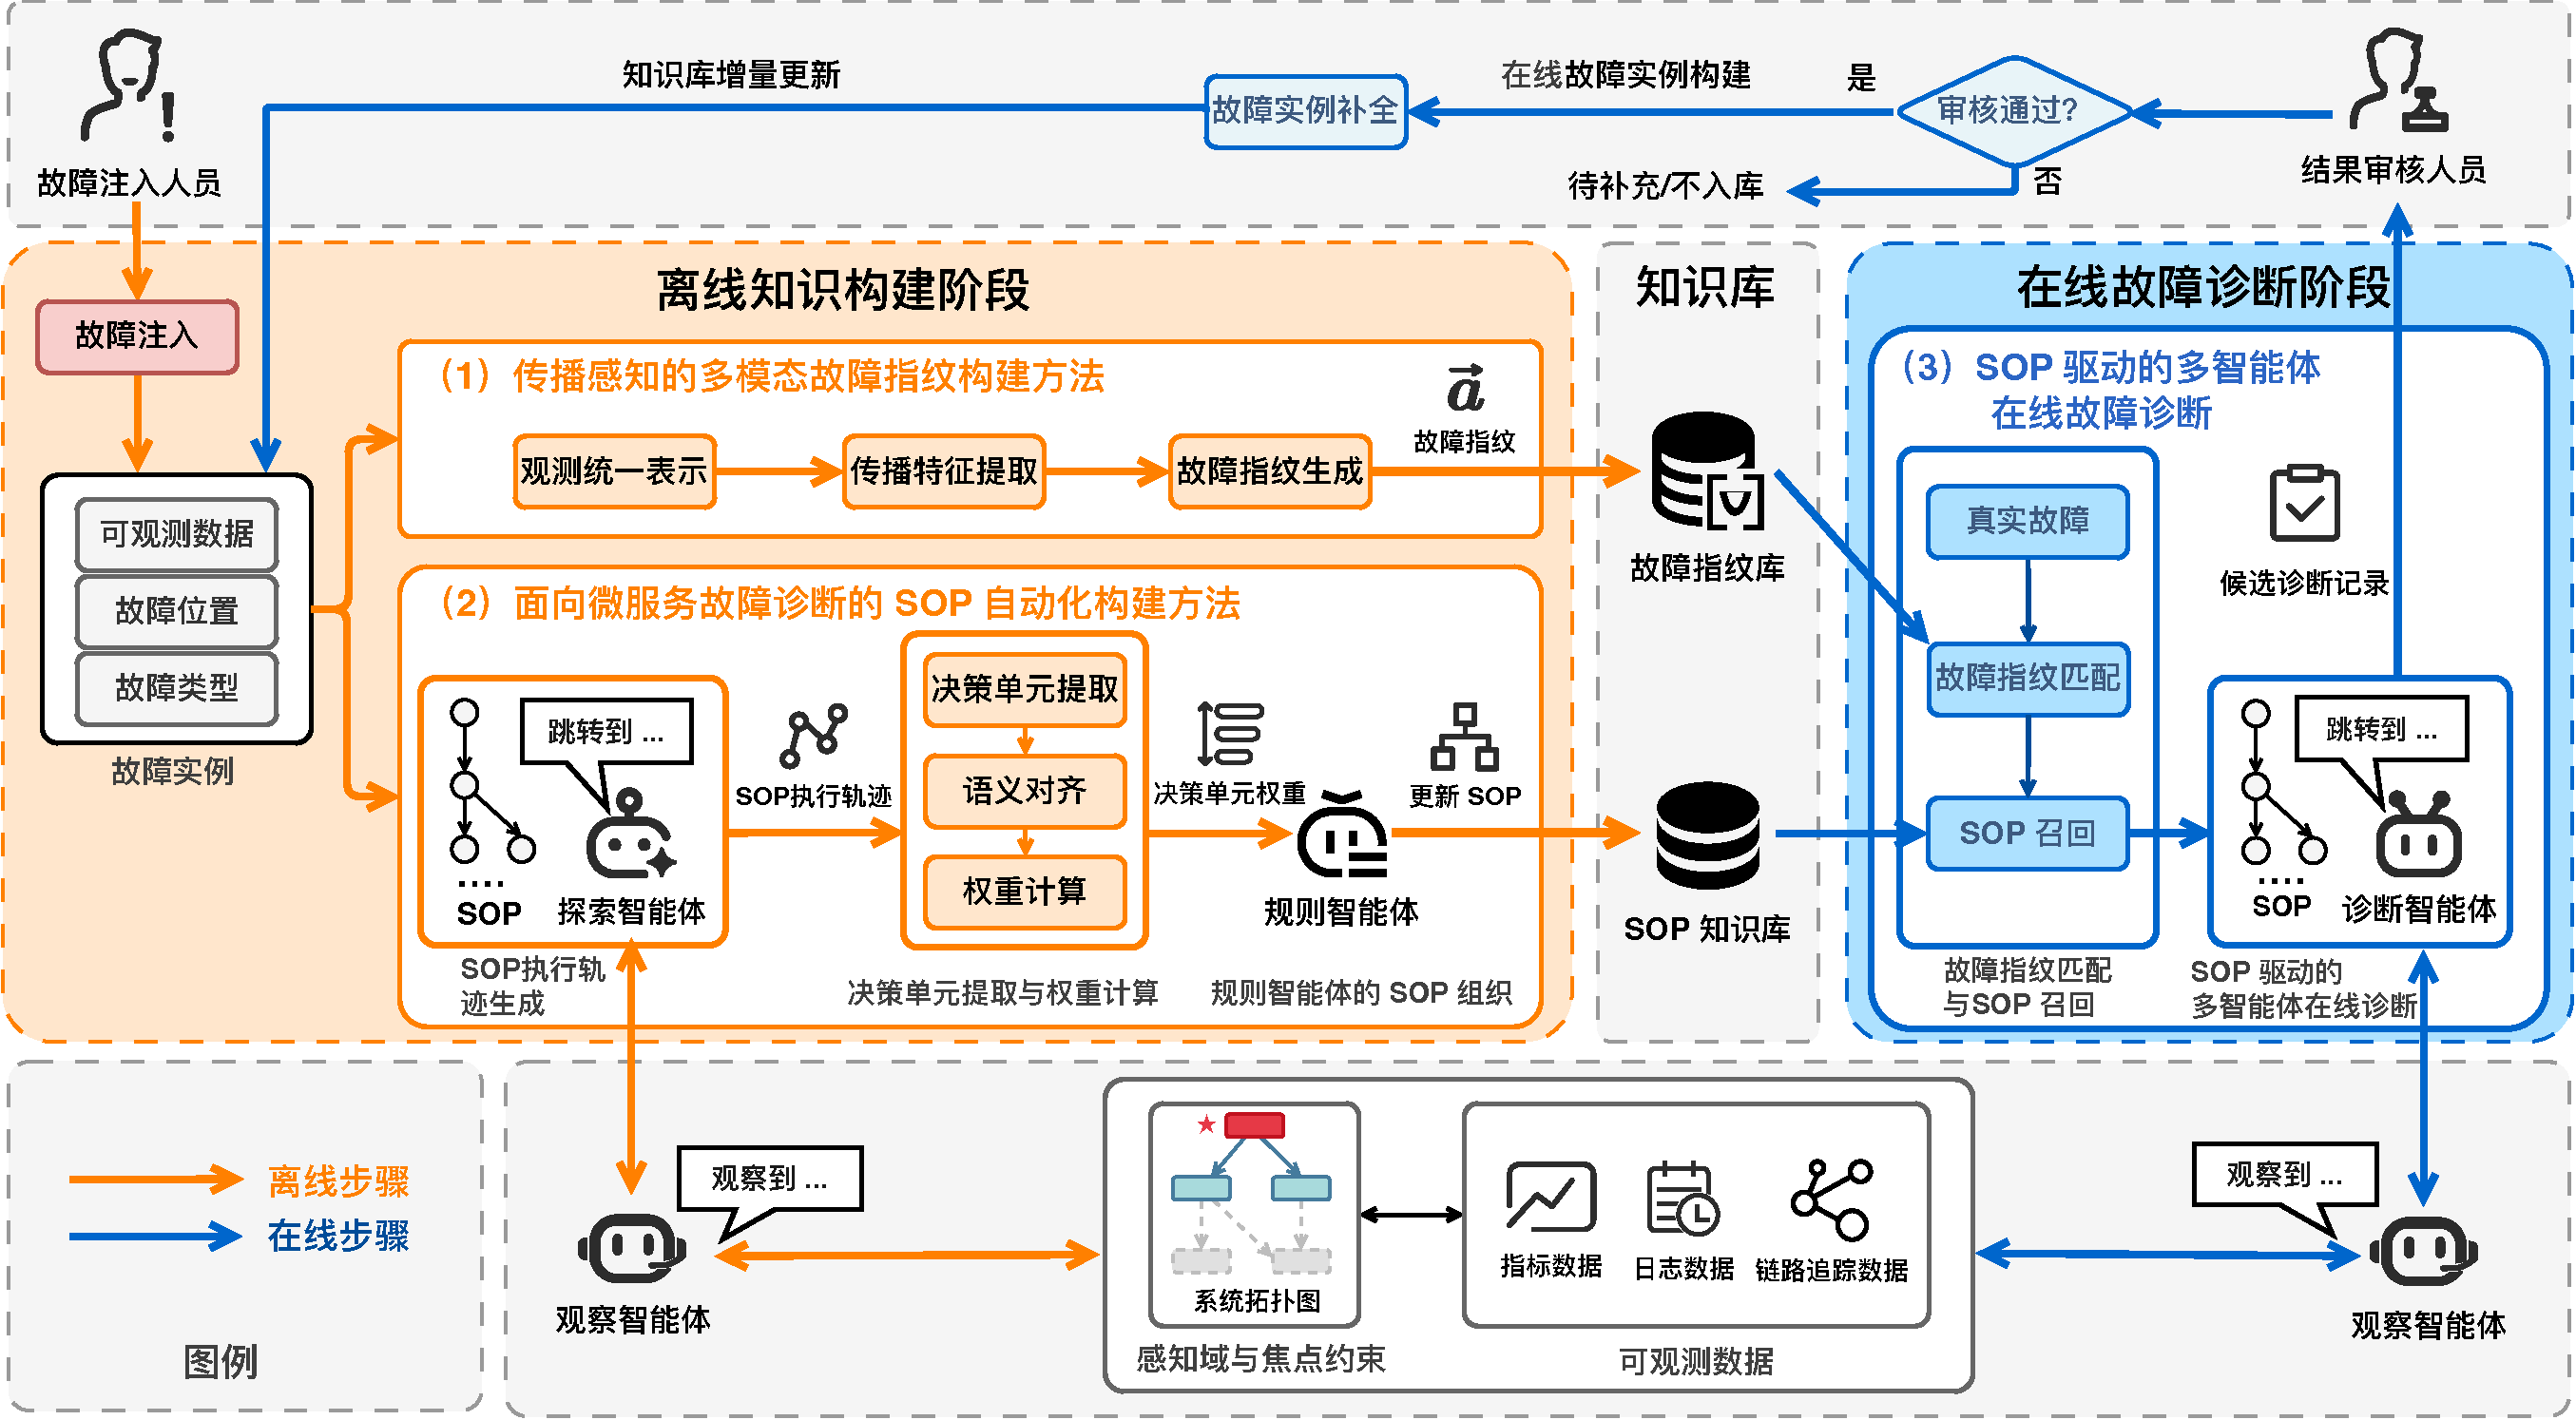
\includegraphics[width=\textwidth]{Figures-Src/Chap3-Methodology/overall-architecture/chart.pdf}
    \bicaption{经验驱动的微服务故障根因定位智能体流程}{Workflow of Experience Driven Agent-Based Root Cause Localization}
    \label{fig:overall_arch}
\end{figure}
\FloatBarrier


\textbf{离线知识构建阶段}以故障注入实验产生的有效故障实例为输入，其中包含故障窗口内的指标、日志、调用链路，以及已知的故障位置和故障类型。该阶段包含两项技术：\textbf{（1）传播感知的多模态故障指纹构建方法（第3.2节）}，用于把多模态观测数据转化为固定维度的故障指纹；\textbf{（2）面向微服务故障诊断的 SOP 自动化构建方法（第3.3节）}，用于从故障实例中生成 SOP执行轨迹、提取决策单元并组织为可执行 SOP。离线阶段完成后，系统形成故障指纹库和 SOP 知识库，分别服务于相似故障检索和在线诊断。

\textbf{在线故障诊断阶段}面向生产环境中的真实故障，对应\textbf{（3）SOP驱动的智能体在线故障诊断方法（第3.4节）}。当新故障发生时，获得当前场景观测数据生成故障指纹，检索故障指纹库中最相似的历史故障簇并召回对应 SOP。诊断智能体与观察智能体在共享观察能力支持下推进排查；若现有 SOP 无法覆盖当前分支，则进入受控逃逸模式，在有限范围内扩展路径。诊断结束后，系统生成候选诊断记录并提交人工审核。审核通过后，该记录作为新的故障实例回流离线阶段，执行故障指纹和 SOP 的增量更新。


%---------------------------------------------------------------------------%
%->> 3.2 传播感知的多模态故障指纹构建方法
%---------------------------------------------------------------------------%
%---------------------------------------------------------------------------%
%->> Section 3.2: 传播感知的多模态故障指纹构建方法
%---------------------------------------------------------------------------%

\section{传播感知的多模态故障指纹构建方法}

ASE 2024 的 FAIL 研究对 2010 年至 2022 年间公开报道的 2457 起软件故障进行了统计，结果表明，其中 85\% 属于重复或相似场景，77\% 会在同一组织内再次出现，53\% 会在不同组织间重复出现\cite{fail-anandayuvaraj2024}。这说明，生产环境中的大量故障并不是孤立事件。历史故障中留下的观测模式和诊断线索，具有直接复用的价值。

然而，在实际运维场景中，历史诊断案例的诊断经验往往难以被直接复用。其核心问题在于，当前故障与历史故障之间缺乏统一的表征框架。现有做法常用工单标题、案例摘要或人工标注的故障类型描述故障，例如“服务超时”，“数据库异常”，“调用链抖动”等。这类描述便于归档，却往往停留在症状层面，难以回答更关键的问题：异常首先出现在哪里、指标如何变化、日志呈现出何种模式，以及异常沿何种依赖关系传播。以“服务超时”为例，它既可能由数据库连接池耗尽引起，也可能源于缓存雪崩或网络抖动；与此同时，不同根因也可能表现出相近的外部症状。这种现象表明，真正具备跨场景复用价值的，并非粗粒度的静态标签，而是故障发生时多模态观测数据所蕴含的细粒度故障模式。

要把这些模式表征出来，难点在于相关线索分散在指标、日志和调用链路中。三类数据的结构、语义层级和特征形式差异很大，不能直接比较。为了使历史诊断经验能够被稳定召回，系统需要为一次故障构建一种同时保留多模态观测特征与传播信息、且便于跨实例比较的统一表示。为此，本文提出故障指纹（Fault Fingerprint）的概念，用固定维度向量表示一次故障窗口内的多模态观测，并以向量距离衡量故障之间的相似性。在此基础上，本文提出传播感知的多模态故障指纹构建方法（Propagation-Aware Multimodal Fault Fingerprinting，PMF）。该方法首先对指标、日志和调用链路进行统一表示；随后围绕故障传播过程提取多模态特征；最后通过标准化与特征筛选生成故障指纹。

\subsection{故障指纹构建方法的设计}

故障指纹主要用于相似故障实例的检索。它的核心目标不是为故障‘贴标签分类’，而是对比当前现象与历史记录在故障演化过程上的相似度。因此，构建故障指纹时需要把握好特征的平衡：既要精准提取出故障形成与传播的核心规律，又要剔除掉特定场景下的偶然干扰（如具体的服务实例名或环境参数），确保提取出的特征具有足够的通用性和跨场景匹配能力。

\begin{figure}[tbp]
    \centering
    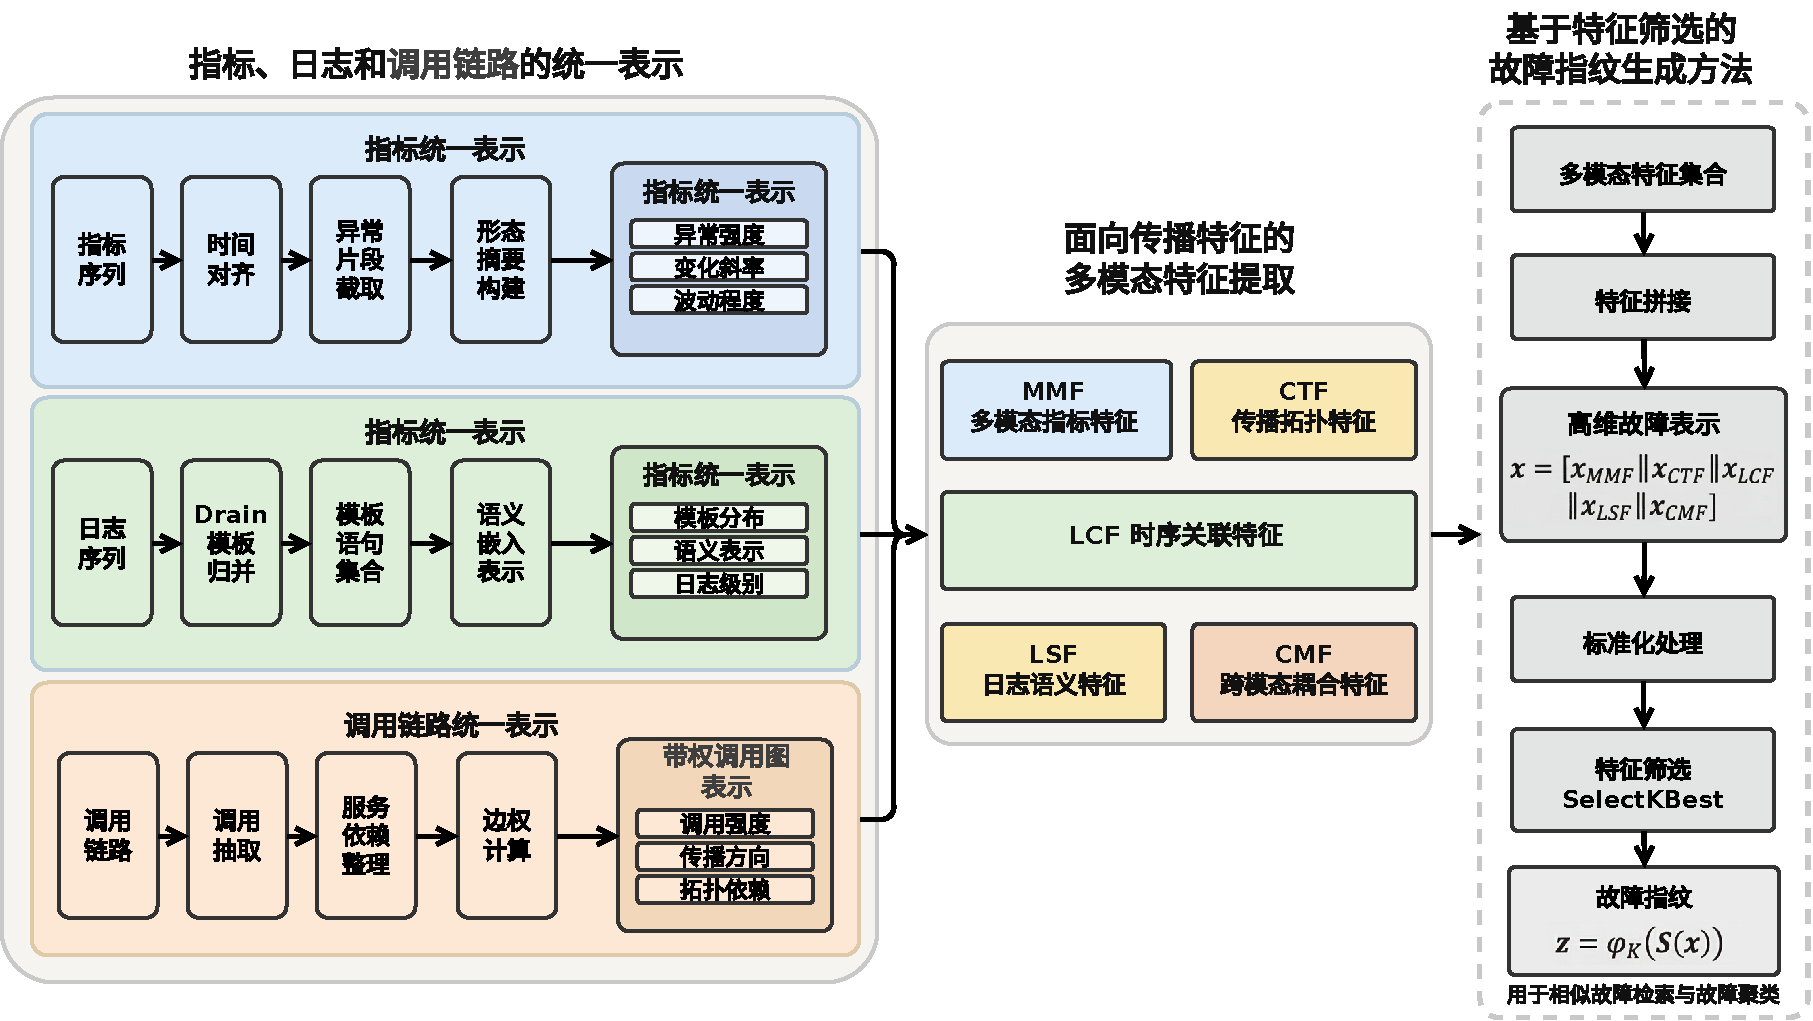
\includegraphics[width=\textwidth]{Figures-Src/Chap3-Methodology/fault-representation/chart.pdf}
    \bicaption{\enspace 传播感知的多模态故障指纹构建流程}{\enspace Pipeline of Propagation-Aware Multimodal Fault Fingerprinting}
    \label{fig:fingerprint_framework}
\end{figure}

图\ref{fig:fingerprint_framework}给出了传播感知的多模态故障指纹构建方法的整体三阶段构建流程。

\begin{enumerate}[label=（\arabic*）]

    \item \textbf{指标、日志和调用链路的统一表示。}  该阶段以故障窗口内的原始指标、日志和服务调用链路为输入，分别形成指标形态摘要、日志模板语义表示和带权服务调用图三类中间表示。其目的不是直接生成故障指纹，而是先将结构、粒度和语义层级不同的观测数据转换为可比较的表示，为后续统一建模提供基础。

    \item \textbf{面向故障传播特征的多模态特征提取。}  该阶段以上一步得到的三类中间表示为输入，进一步提取多模态指标特征、传播拓扑特征、时序关联特征、日志语义特征和跨模态耦合特征。其作用是在统一表示基础上，保留真正与故障传播过程相关的信息，使故障表示不仅反映局部异常，还能够体现传播路径、上下游影响和跨模态联动关系。

    \item \textbf{基于特征筛选的故障指纹生成方法。}  该阶段以高维多模态特征为输入，通过标准化与特征筛选生成固定维度的故障指纹。其作用是从大量候选特征中保留更具稳定性和区分能力的部分，使最终表示既能保留故障传播特征，又适合用于相似故障检索与历史经验绑定。
\end{enumerate}

以下示例有助于进一步理解设计要点。\textit{某电商系统在不同时间发生的两次支付超时故障。第一次故障由数据库连接池耗尽引起，表现为数据库连接错误日志出现、支付服务响应时延持续升高，并进一步导致上游订单服务超时；第二次故障由缓存服务宕机引起，表现为缓存不可用、数据库查询压力激增以及支付服务时延上升}。两次故障在入口症状上都表现为“支付超时”，但其内部形成过程并不相同。若仅依赖工单标题或故障标签，系统很容易将二者归为同一类故障，进而匹配到并不合适的历史排查经验。相反，若故障表示能够同时保留日志线索、指标变化和传播路径，那么这两次故障在表示空间中应当具有可区分性。

基于这一考虑，本文将\textbf{故障指纹}定义为：在故障窗口期内，从指标、日志和服务调用拓扑中提取的、用于相似故障检索的固定维度嵌入向量。若两个故障事件在故障指纹空间中的距离较近，则表明二者在微服务上下文、观测模式和传播特征上更为相似，因而更可能对应相同或相近的故障形成过程；若距离较远，则说明其内部模式存在较大差异。

本文将一次故障定义为一个故障事件，表示为
\begin{equation}
\mathcal{E}=\langle \mathcal{M}, \mathcal{L}, \mathcal{G}\rangle
\end{equation}
其中，$\mathcal{M}$ 表示故障窗口期内的指标集合，$\mathcal{L}$ 表示日志集合，$\mathcal{G}$ 表示服务调用拓扑。故障指纹构建即是定义映射函数
\begin{equation}
\mathbf{z}=F(\mathcal{E}), \quad \mathbf{z}\in\mathbb{R}^{K}
\end{equation}
其中，$\mathbf{z}$ 表示故障事件 $\mathcal{E}$ 对应的故障指纹。

对于任意两个故障事件 $\mathcal{E}_i$ 与 $\mathcal{E}_j$，理想情况下，若二者对应相同或相近的故障，则其故障指纹表示应更接近；若二者的故障形成过程存在显著差异，则其故障指纹表示应保持分离性。为了使映射 $F$ 满足这一要求，本文对故障指纹构建提出如下两点设计要求：

\begin{itemize}
    \item \textbf{稳定性。} 即指纹的提取必须过滤掉特定服务实例名、环境参数或局部瞬时波动的干扰，确保相同成因的故障在不同的请求、实例和流量背景下，仍能稳定映射为相近的表示；
    
    \item \textbf{可区分性。} 即指纹不能仅停留在粗粒度的表面症状层面，而应深入保留故障演变与传播的关键线索，从而能够准确区分那些“入口症状相近但内部成因完全不同”的故障。
\end{itemize}

故障指纹构建映射 $F$涉及可观测数据的统一表征、面向传播特征的多模态特征提取和基于特征筛选的故障指纹生成，下面分别进行详细阐述。

\subsection{指标、日志和调用链路的统一表示}

故障窗口内的原始观测包括指标、日志和调用链路数据。三类数据在表示形式和统计特征上差异很大：指标是连续采样的时间序列，日志是包含大量变量和上下文的离散文本流，调用链路则体现为服务之间的调用关系及其结构依赖。如果直接将它们拼接到一起，不仅会带入大量与故障特征无关的实例级细节，也难以建立跨故障稳定比较的基础。因此，本文先分别对三类观测进行统一表示，得到三类中间表示，为后续特征提取提供输入。

\textbf{指标形态摘要。}
对指标数据而言，关键并不是保留完整时间序列，而是抓住故障期间的变化形态。为此，本文以“服务$\times$指标”二元组为基本统计单元，在故障窗口内完成时间对齐，并提取异常强度、变化斜率、跃迁幅度、波动性和尖峰比例等统计量。用于比较的并不是某一时刻的精确取值，而是故障期间是否出现了持续升高、快速跃迁、剧烈波动或尖峰突发等模式。例如，数据库连接池耗尽通常表现为连接数持续升高并逼近上限，网络抖动则更常表现为时延的明显波动。经过这一步，原始指标序列被压缩为相对稳定的形态摘要，从而减弱负载波动、采样频率差异和局部瞬时扰动对比较结果的影响。

\textbf{日志模板与语义表示。}
日志数据的难点主要在于表面表达离散，而且容易受到实例变量干扰。相同故障在不同实例中留下的日志往往语义相近，但文本形式并不相同，例如“Connection timeout to DB instance db-01”和“Connection timeout to DB instance db-02”。为此，本文首先采用 He 等提出的 Drain 在线日志解析算法~\cite{drain-he2018}，将原始日志归并为模板序列。Drain 通过固定深度的解析树，将日志文本中的变量部分替换为通配符，从而将上述两条日志统一归并为模板“Connection timeout to DB instance <*>”。

在模板归并之后，本文进一步采用预训练语义嵌入模型对模板文本进行编码：
\begin{equation}
\mathbf{e}_k = f_{\text{emb}}(T_k)
\end{equation}
其中，$T_k$ 表示日志模板，$\mathbf{e}_k$ 表示对应的模板语义向量。这样做的目的，是将语义相近但表面表述不同的日志模式映射到更为接近的语义空间区域。例如，“Connection timeout”和“Database connection failed”虽然文本不同，但在语义空间中的距离较近，因此可以被识别为相近的错误模式。如图\ref{fig:drain_parsing}所示，原始日志在解析树中按层次逐步匹配，并最终归并至相应模板，从而将实例标识、请求编号和变量取值等高频变化项从日志主体中分离出来。经过这一处理后，日志观测被转换为更适合跨故障比较的日志模板及其语义表示。

\begin{figure}[tbp]
    \centering
    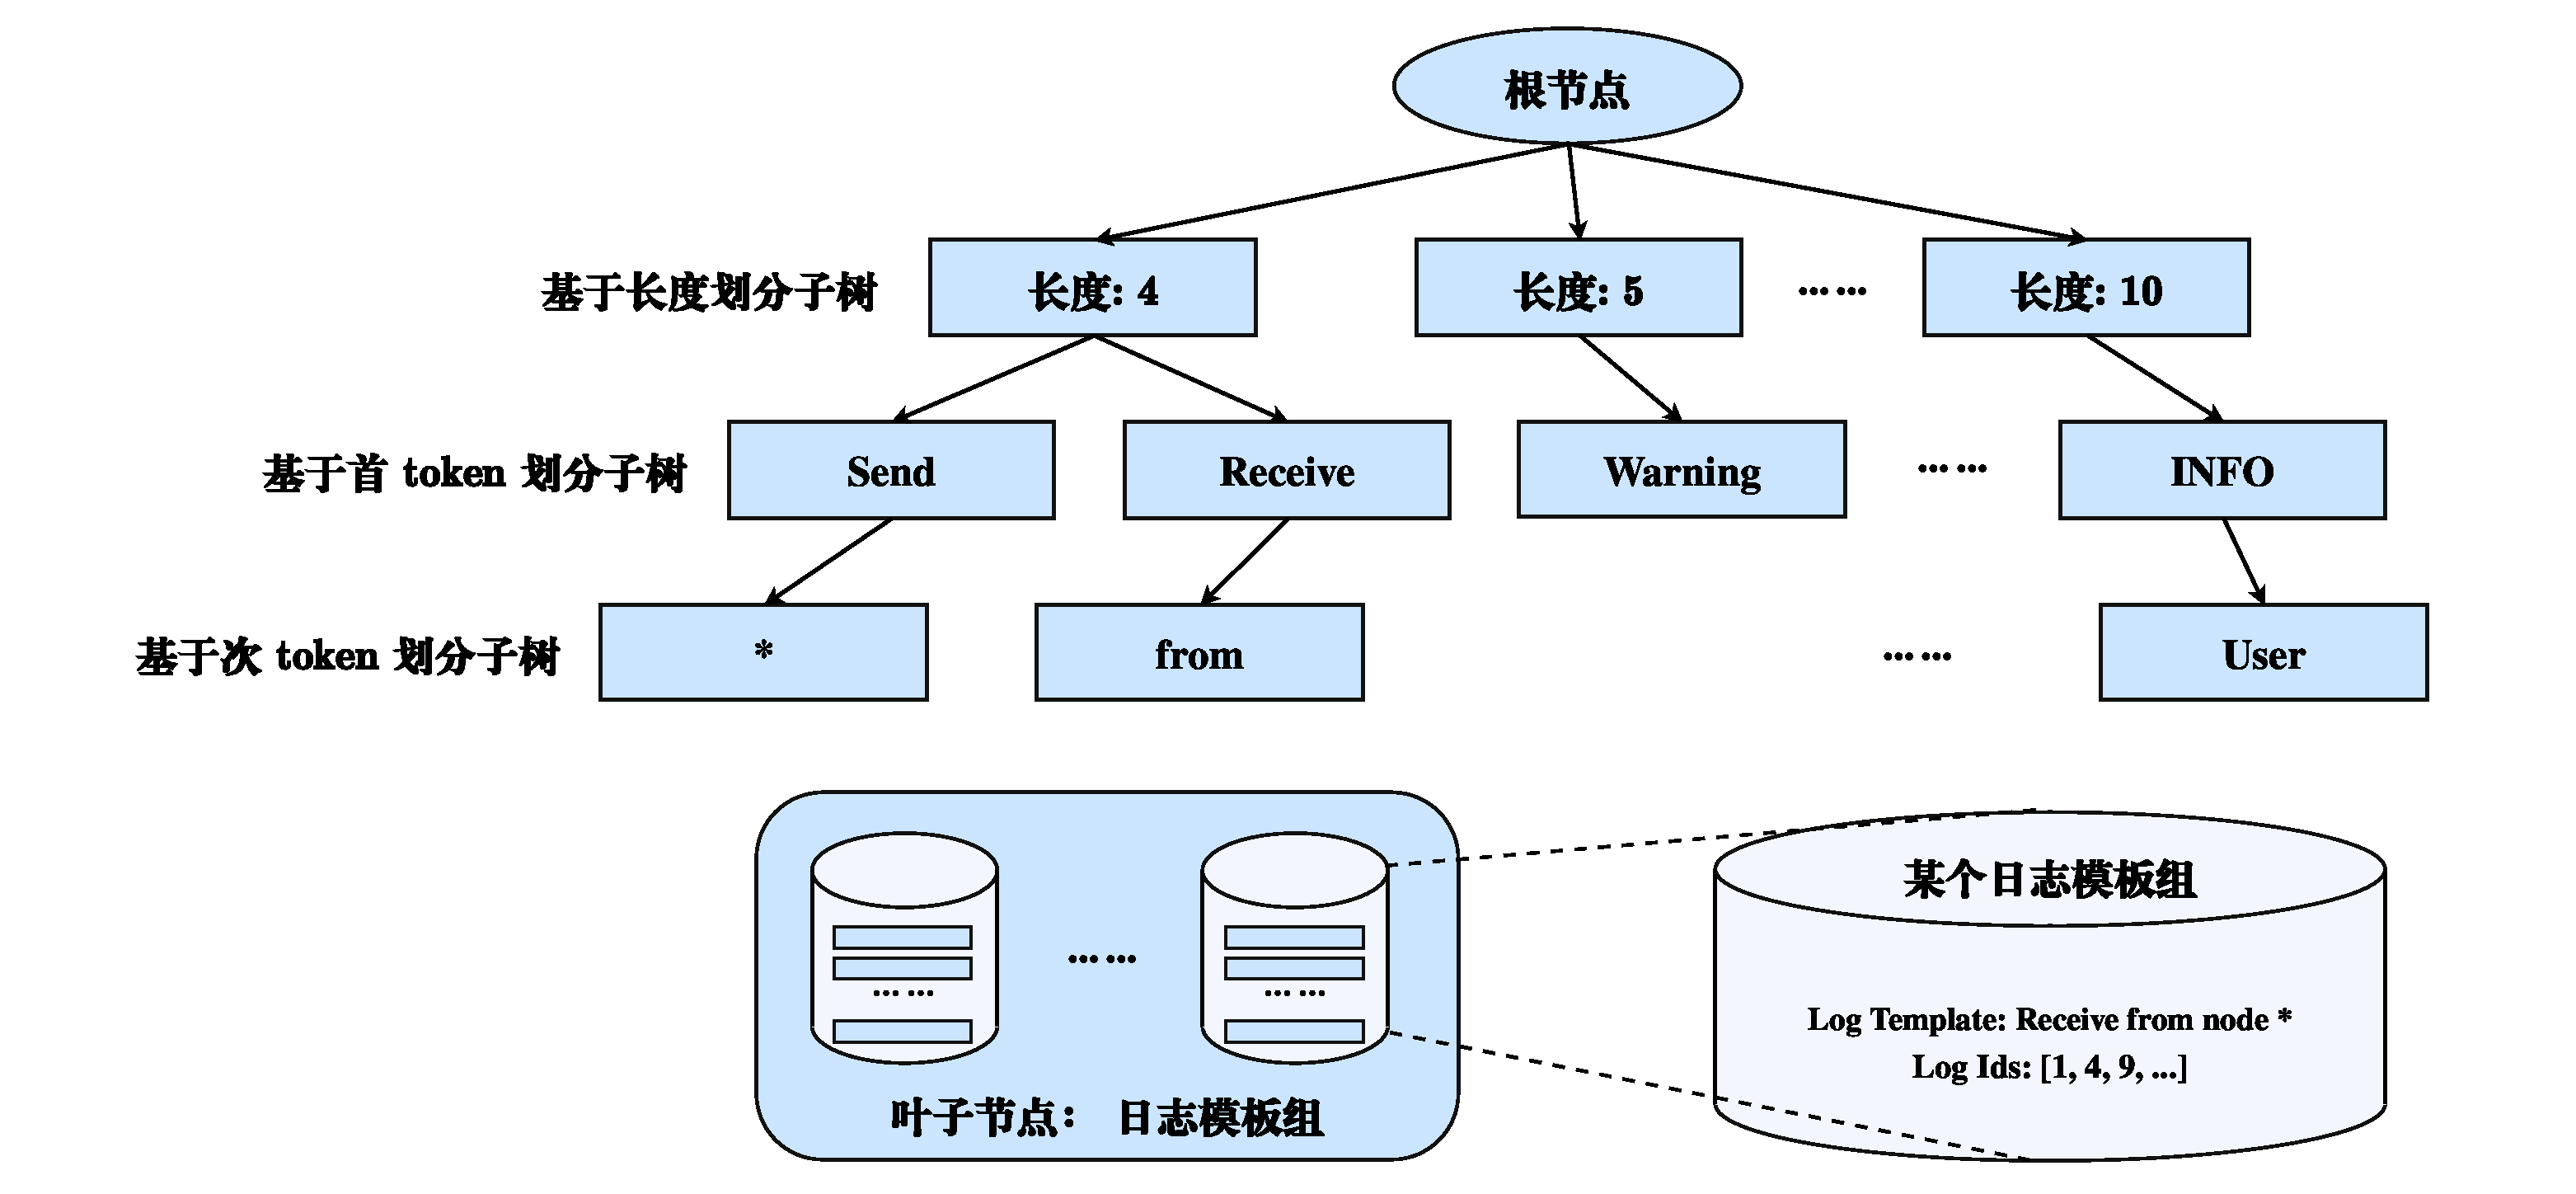
\includegraphics[width=0.9\textwidth]{Figures-Src/Chap3-Methodology/drain/chart.pdf}
    \bicaption{\enspace Drain日志模板解析与模板归并}{\enspace Drain-based Log Template Parsing and Template Grouping}
    \label{fig:drain_parsing}
\end{figure}

\textbf{带权服务调用图。}
调用链路部分保留的是故障的结构上下文。微服务故障通常不会停留在某一个服务内部，而会沿着服务依赖关系向上下游传播。例如，数据库连接池耗尽可能先导致数据访问层服务响应变慢，继而引发业务逻辑层服务超时，最终传播到前端 API 服务。不同故障之间的差异，不仅体现在哪些服务出现异常，还体现在异常沿哪条依赖链演化、哪些节点处于关键传播位置，以及上下游耦合强度如何变化。为此，本文从调用链路数据中提取服务间调用边，构建服务级调用图 $G=(V,E)$，并以故障窗口内的调用计数$c_{i,j}$作为边$(i,j)$ 的原始权重。其中，节点表示服务实体，边的原始权重反映服务之间的调用频次。该有向图及其原始边权共同保留了传播方向和耦合强度，并为后续多模态特征提取提供统一输入。在后续传播拓扑特征提取阶段，本文再基于这些原始边权进行归一化处理，并计算传播相关统计量。

经过上述处理，原始指标、日志和调用链路分别被表示为指标形态摘要、日志模板及其语义表示，以及带权服务调用图。这些中间表示构成了后续传播特征提取的输入。

\subsection{面向传播特征的多模态特征提取}

统一表示之后，跨故障比较的基础已经建立，但最终检索效果仍取决于所保留特征是否真正与故障传播过程相关。若直接将三类中间表示拼接，虽然能够保留部分信息，但仍然难以突出传播路径、时序联动和跨模态协同等关键因素。为此，本文围绕指标异常、传播结构、时序关系、日志语义和跨模态耦合提取五类特征。考虑到服务组合、调用边和日志模板数量较多，本文对高频项直接保留其统计特征，对低频组合采用固定维度哈希编码，以避免特征维度随系统规模增长而持续膨胀。

\textbf{指标形态特征（Metric Morphology Features，MMF）。}
MMF 是故障指纹中描述指标模态异常形态的特征分量。本文首先统计高频服务和高频指标的异常强度分布，再对每个”服务$\times$指标”组合计算平均强度、变化斜率、跃迁幅度、波动性和尖峰比例。对于出现次数较少的服务--指标组合，则采用固定维度哈希编码保留其异常信息。该类特征主要用于区分资源持续升高、局部性能抖动和短时突发波动等不同类型的指标异常。

\textbf{传播拓扑特征（CTF）。}
CTF 用于刻画异常在服务依赖结构中的传播组织方式。微服务故障通常不会停留在单一服务内部，而会沿上下游依赖关系扩散。因此，异常扩散涉及哪些边、哪些节点处于传播中心、哪些区域承载更高扩散风险，都应作为故障表示的重要组成部分。设故障窗口内调用边 $(i,j)$ 的调用计数为 $c_{ij}$，则其归一化权重记为
\begin{equation}
a_{ij}=
\begin{cases}
\dfrac{c_{ij}}{\sum_{(p,q)\in E} c_{pq}}, & (i,j)\in E \\
0, & \text{otherwise}
\end{cases}
\end{equation}
在此基础上，分别计算节点的入度 $d_i^{\text{in}}$ 与出度 $d_i^{\text{out}}$，并定义拓扑中心性与传播倾向：
\begin{equation}
c_i^{\text{topo}} = d_i^{\text{in}} + d_i^{\text{out}}
\end{equation}
\begin{equation}
p_i^{\text{prop}} = \frac{d_i^{\text{out}}}{d_i^{\text{in}} + d_i^{\text{out}} + \epsilon}
\end{equation}
其中，拓扑中心性反映服务在传播结构中的连接程度，传播倾向衡量异常继续向下游扩散的可能性。为了进一步估计异常在整张调用图上的传播范围，本文使用带权随机游走计算故障传播影响力，并针对微服务故障传播的连续带权特性做三项调整。若服务 $i$ 对应节点 $v_i$，则节点影响力初始化不采用均匀分布，而是由节点上的故障严重程度决定：
\begin{equation}
r_i^{(0)} = \frac{\text{severity}(v_i)}{\sum_{v_j \in V} \text{severity}(v_j)}
\end{equation}
转移概率由调用边权重定义：
\begin{equation}
W_{ij} = \frac{c_{ij}}{\sum_{k \in \text{out}(i)} c_{ik}}
\end{equation}
同时，引入时间衰减因子刻画传播时序性：
\begin{equation}
\mathbf{r}^{(t+1)} = (1-\alpha) \mathbf{W}^{\top}(\mathbf{r}^{(t)} \odot \boldsymbol{\beta}^{\Delta t}) + \frac{\alpha}{|V|}\mathbf{1}
\end{equation}
其中，$\mathbf{W}$ 为按出边归一化后的带权转移矩阵，$\alpha$ 为阻尼系数，$\boldsymbol{\beta}^{\Delta t}$ 为时间衰减因子向量，$\odot$ 表示逐元素乘法，$\mathbf{r}$ 为服务影响力向量。经过上述处理，CTF 由边频次统计、入出度分布、全局结构统计、拓扑中心性、传播倾向和传播影响力共同构成，用于描述故障围绕哪些关键节点展开，以及异常可能沿哪些依赖链继续扩散。

\textbf{时序关联特征（LCF）。}
LCF 用于区分“结构上可能传播”和“运行时确实联动”这两种不同情形。静态调用链路只能说明服务之间存在传播路径，并不能证明故障在当前窗口内真的沿该路径扩散。为此，本文在服务级别对指标信号与日志信号进行分钟级聚合，并在有限滞后窗口内搜索最优相关性：
\begin{equation}
\rho_i = \max_{\ell \in [-L,L]} \left|\operatorname{corr}\left(m_i(t), l_i(t+\ell)\right)\right|
\end{equation}
其中，$m_i(t)$ 表示服务 $i$ 的指标信号，$l_i(t)$ 表示服务 $i$ 的日志信号，$\ell$ 表示滞后步长。除最优相关性外，本文还保留最优滞后位置、滞后直方图和整体统计结果，用于描述不同服务中“指标异常领先日志”或“日志异常领先指标”的时序关系。LCF 为拓扑上的潜在传播关系补充了时间证据，从而避免仅凭结构邻接关系误判真实传播链。

\textbf{日志语义特征（Log Semantic Features，LSF）。}
LSF 用于从模板分布和时间强度两个方面刻画日志异常，其处理对象为故障窗口内经 Drain 解析后得到的日志模板序列。具体而言，系统统计各模板的出现频次及分布，提取 ERROR、WARN、INFO 各级别日志的占比，并计算故障窗口内的日志突发强度（单位时间内的异常等级日志数量）。由于统一表示阶段已经引入模板语义嵌入，不同文本表达但语义相近的模板能够在统一语义空间中对齐，因此 LSF 同时保留模板频次及语义归一化后的统计结果，使日志异常模式在跨故障比较中具有语义一致性。

\textbf{跨模态耦合特征（Cross-Modal Coupling Features，CMF）。}
CMF 用于刻画指标、日志和调用链路之间的联动关系，其基本假设是真实故障往往在多个模态中同时留下异常信号。在指标—日志联动层面，系统计算服务粒度上指标异常出现时间与日志异常出现时间的时差分布；在链路—日志联动层面，统计调用边上时延升高事件与下游异常日志事件的共现比例。此外，CMF 综合统计服务数、指标种类数、日志量、上下游服务规模、平均边权、异常强度和日志错误比例等全局规模变量，并进一步计算传播风险分数，以反映异常规模、传播范围与日志响应强度是否呈现一致增强，从而区分真实多模态联动故障与单模态假阳性事件。

基于上述三类中间表示，本文提取了 MMF、CTF、LCF、LSF 和 CMF 五类特征。MMF 描述故障在指标层面的异常形态，CTF 和 LCF 刻画传播结构及其时序证据，LSF 提供日志层面的补充信息，CMF 反映不同模态之间是否存在一致的异常增强现象。这五类特征共同构成后续故障指纹生成的输入。

\subsection{基于特征筛选的故障指纹生成方法}

经过统一表示与传播特征提取两个阶段后，一次微服务故障已经被表示为五类面向传播特征的高维特征。但这些特征还不能直接作为最终故障指纹用于相似故障检索，因为不同特征块在数值范围、稀疏程度和统计稳定性上存在明显差异。例如，指标特征通常表现为连续数值，日志特征则往往是高度稀疏的计数；同时，也存在部分特征维度在不同故障之间缺乏足够区分能力。若将所有特征不加选择地保留到最终表示中，故障指纹将包含较多冗余特征和弱相关特征，从而削弱相似故障在表示空间中的聚合效果。

为此，本文首先将五类特征拼接为统一的高维故障表示：
\begin{equation}
\mathbf{x} =
\left[
\mathbf{x}^{\text{MMF}} \,\Vert\,
\mathbf{x}^{\text{CTF}} \,\Vert\,
\mathbf{x}^{\text{LCF}} \,\Vert\,
\mathbf{x}^{\text{LSF}} \,\Vert\,
\mathbf{x}^{\text{CMF}}
\right]
\end{equation}
其中，$\Vert$ 表示向量拼接操作。由于不同特征块在量纲和分布上存在显著差异，本文先对拼接后的特征向量进行标准化处理，以减弱数值范围差异对后续判别过程的影响。

在此基础上，为保留对故障区分更有贡献的特征，本文采用单变量方差分析的 \texttt{SelectKBest} 方法对高维特征进行筛选~\cite{scikit-learn,scipy}，记筛选映射为 $\phi_K(\cdot)$。最终故障指纹定义为
\begin{equation}
\mathbf{z} = \phi_K(\tilde{\mathbf{x}})
\end{equation}
其中，$\tilde{\mathbf{x}}$ 表示标准化后的高维特征向量，$\mathbf{z}$ 表示筛选后的故障指纹。通过该步骤，最终表示在保留多模态关键信息的同时，减少了低价值维度的干扰，从而提高故障指纹的判别性与检索稳定性。


\makeatletter
\@addtoreset{algorithm}{chapter}
\setlength{\@fptop}{0pt}
\makeatother
\renewcommand{\thealgorithm}{\thechapter-\arabic{algorithm}}
\floatname{algorithm}{算法}

\algrenewcommand\algorithmicrequire{\textbf{输入：}}
\algrenewcommand\algorithmicensure{\textbf{输出：}}
\algrenewcommand\algorithmicforall{\textbf{对每个}}
\algrenewcommand\algorithmicdo{\textbf{执行}}
\algrenewcommand\algorithmiccomment[1]{\hfill// #1}
\algtext*{EndFor}

\begin{algorithm}[!t]
    \caption{\enspace PMF 故障指纹构建算法}
    \label{alg:fault_fingerprint}
    \begin{algorithmic}[1]
        \Require 训练故障集 $\mathcal{D}=\{\mathcal{E}_i\}_{i=1}^{N}$，保留维度 $K$，相关性阈值 $\rho_{\max}$
        \Ensure 故障指纹映射 $F(\cdot)$
        \State InitEncoding($\mathcal{D}$) \Comment{初始化高频统计项与低频组合的哈希编码规则}
        \ForAll{故障事件 $\mathcal{E}_i \in \mathcal{D}$}
            \State $\mathbf{m}_{\mathcal{E}_i} \leftarrow$ BuildMetrics($\mathcal{E}_i$) \Comment{构造指标形态摘要}
            \State $\mathbf{l}_{\mathcal{E}_i} \leftarrow$ BuildLogs($\mathcal{E}_i$) \Comment{构造日志模板及其语义表示}
            \State $G_{\mathcal{E}_i} \leftarrow$ BuildCalls($\mathcal{E}_i$) \Comment{构造服务级调用图}
            \State $(\mathbf{x}^{\mathrm{MMF}}_{\mathcal{E}_i},\mathbf{x}^{\mathrm{CTF}}_{\mathcal{E}_i},\mathbf{x}^{\mathrm{LCF}}_{\mathcal{E}_i},\mathbf{x}^{\mathrm{LSF}}_{\mathcal{E}_i},\mathbf{x}^{\mathrm{CMF}}_{\mathcal{E}_i})$
            \State \hspace{1.5em} $\leftarrow$ ExtractFeatures($\mathbf{m}_{\mathcal{E}_i},\mathbf{l}_{\mathcal{E}_i},G_{\mathcal{E}_i}$) \Comment{提取五类传播特征}
            \State $\mathbf{x}_{\mathcal{E}_i} \leftarrow$ ConcatFeatures$(\mathbf{x}^{\mathrm{MMF}}_{\mathcal{E}_i},\mathbf{x}^{\mathrm{CTF}}_{\mathcal{E}_i},\mathbf{x}^{\mathrm{LCF}}_{\mathcal{E}_i},\mathbf{x}^{\mathrm{LSF}}_{\mathcal{E}_i},\mathbf{x}^{\mathrm{CMF}}_{\mathcal{E}_i})$ \Comment{拼接得到高维故障表示}
        \EndFor
        \State $\mathbf{X} \leftarrow$ StackMatrix$(\{\mathbf{x}_{\mathcal{E}_i}\}_{i=1}^{N})$ \Comment{构造特征矩阵}
        \State $S \leftarrow$ FitNormalizer$(\mathbf{X})$ \Comment{拟合标准化映射}
        \State $\tilde{\mathbf{X}} \leftarrow S(\mathbf{X})$ \Comment{得到标准化特征矩阵}
        \State $\mathbf{s} \leftarrow$ ComputeVarianceScore$(\tilde{\mathbf{X}})$ \Comment{计算各维特征的方差得分}
        \State $\mathcal{S}_{K} \leftarrow$ SelectFeatures$(\mathbf{s},\tilde{\mathbf{X}},K,\rho_{\max})$ \Comment{按得分排序并结合相关性约束保留 $K$ 维特征}
        \State 定义故障指纹映射 $F(\mathcal{E})=\left(S(\mathbf{x}_{\mathcal{E}})\right)_{\mathcal{S}_{K}}$
        \State \Return $F(\cdot)$
    \end{algorithmic}
\end{algorithm}



算法\ref{alg:fault_fingerprint}给出了 PMF 的离线构建过程。该过程首先基于训练故障集完成指标、日志和调用链路的统一表示与传播特征提取，随后通过标准化与特征筛选学习故障指纹映射。该映射可用于后续故障实例的指纹生成，并进一步支持相似故障检索、故障聚类和 SOP 绑定。



%---------------------------------------------------------------------------%
%->> 3.3 SOP自动化构建方法
%---------------------------------------------------------------------------%
%---------------------------------------------------------------------------%
%->> Section 3.3: 面向微服务故障诊断的SOP自动化构建方法
%---------------------------------------------------------------------------%

\section{面向微服务故障诊断的SOP自动化构建方法}

在完成历史故障的统一表示与相似检索之后，系统已经能够从故障指纹库中召回与当前场景相近的历史故障实例。然而，相似实例只能回答“过去发生了什么”，却不能直接回答“当前应如何排查”。对在线诊断而言，真正需要的不只是可供参考的历史案例，还需要一套能够被智能体直接执行的标准操作规程（Standard Operating Procedure，SOP），用于明确排查入口、检查顺序、分支转移条件以及终止判据。

因此，离线知识构建阶段除了构建故障指纹库，还需要进一步把历史故障整理为面向在线诊断的 SOP。这里的关键困难在于：故障实例记录的是故障窗口内的多模态观测结果及最终根因，但并不包含完整的诊断过程；而 SOP 需要显式回答“先检查什么”“依据什么转向”“在什么条件下结束排查”。故障实例与可执行 SOP 之间由此缺少一层能够承接诊断过程的中间表示。围绕这一问题，本文将 SOP 自动化构建组织为如下链路：
\[
\text{故障实例} \rightarrow \text{SOP执行轨迹} \rightarrow \text{决策单元} \rightarrow \text{SOP}.
\]
系统首先围绕历史故障实例执行多轮离线探索，生成带有成功或失败标记的 SOP执行轨迹，把原本缺失的排查步骤、证据依据和路径转移过程显式记录下来；随后从多条轨迹中识别反复出现且能够推动诊断收敛的局部判断，并通过语义对齐和历史统计得到带权决策单元；最后由规则智能体（RuleAgent）结合当前版本 SOP、带权决策单元和代表性轨迹，对 SOP 进行增量更新，形成可供在线诊断直接执行的有向无环图结构。经过这一构建过程，历史故障中的排查经验被逐步整理为能够持续积累和反复调用的结构化诊断知识。

\subsection{SOP构建问题分析与方法设计}

SOP 的价值不在于复述某一次故障，而在于把一次排查中有效的判断依据和路径选择整理为后续同类故障可复用的执行流程。现有运维实践中，这类流程通常由专家根据故障复盘、工单记录和个人经验手工整理，并在系统运行过程中持续更新。这种方式在规模较小、结构相对稳定的系统中仍可工作，但在微服务场景下会迅速暴露出更明显的局限性：

\begin{itemize}
    \item \textbf{排查范围广，人工整理成本高。} 微服务系统通常包含大量服务与复杂依赖关系，一次故障排查往往会跨越多个组件与调用链，人工方式难以稳定覆盖不同场景。
    \item \textbf{系统演化快，流程更新滞后。} 随着部署拓扑、调用关系和故障模式持续变化，人工维护的 SOP 很容易落后于系统实际状态，难以及时反映新的故障传播路径与排查分支。
    \item \textbf{经验环境依赖强，复用性有限。} 人工总结的流程常常绑定具体服务名、实例名或配置细节，在迁移到新环境时仍需重新调整，难以沉淀为稳定的通用诊断知识。
\end{itemize}

在本文的离线阶段中，故障实例主要来自受控的故障注入实验。系统能够获得故障窗口内的指标、日志和调用链路，以及最终确认的故障位置与故障类型。真正的难点不在于收集故障实例，而在于由故障窗口内的观测数据和最终诊断结论推导出合理的排查路径。故障实例能够说明系统在故障窗口内出现了哪些异常、最终根因位于何处，却不能说明排查时先检查了哪些对象、依据什么证据切换方向，以及在何种条件下结束排查。以数据库连接池耗尽为例，一次故障注入实验可以记录支付服务连接错误日志、订单服务响应时延升高、网关请求超时、数据库连接数达到上限，并最终确认根因位于数据库连接池；但这些信息仍不足以还原一条可执行的排查路径。

\begin{figure}[!htbp]
    \centering
    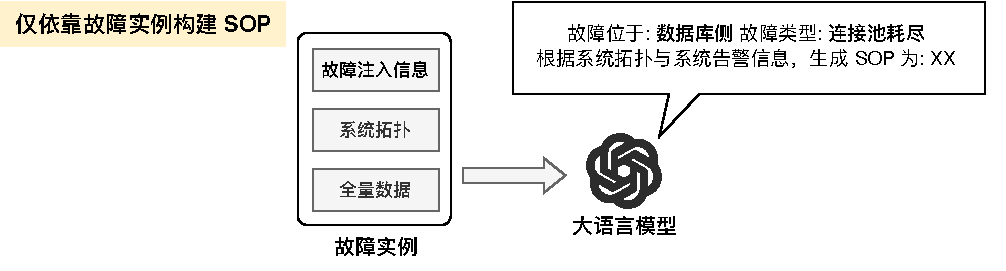
\includegraphics[width=0.82\textwidth]{Figures-Src/Chap3-Methodology/sop-construction-directly/chart.pdf}
    \bicaption{\enspace 由故障实例直接生成SOP的示意}{\enspace Illustration of Direct SOP Generation from Fault Instances}
    \label{fig:sop_direct_generation}
\end{figure}

为了从故障实例中生成可执行的排查路径，一种直观的做法是将故障实例及其相关上下文组织为提示输入，借助大语言模型直接生成 SOP，如图\ref{fig:sop_direct_generation}所示。但这种方法的主要问题在于，模型获得的仍然只是故障观测和最终诊断结论，而中间的排查步骤并未被显式记录，只能由模型根据结果反向推断。因此，生成得到的流程本质上属于基于结果的事后推断。即便这些步骤在表述上看似连贯，其中的检查顺序、转移条件和终止判据仍缺乏真实诊断过程的执行依据，模型甚至可能将故障传播过程中的伴生现象误判为关键诊断线索。对于需要在线执行的诊断系统，仅依赖这种生成方式，难以获得稳定可靠的 SOP。

\begin{figure}[!htbp]
    \centering
    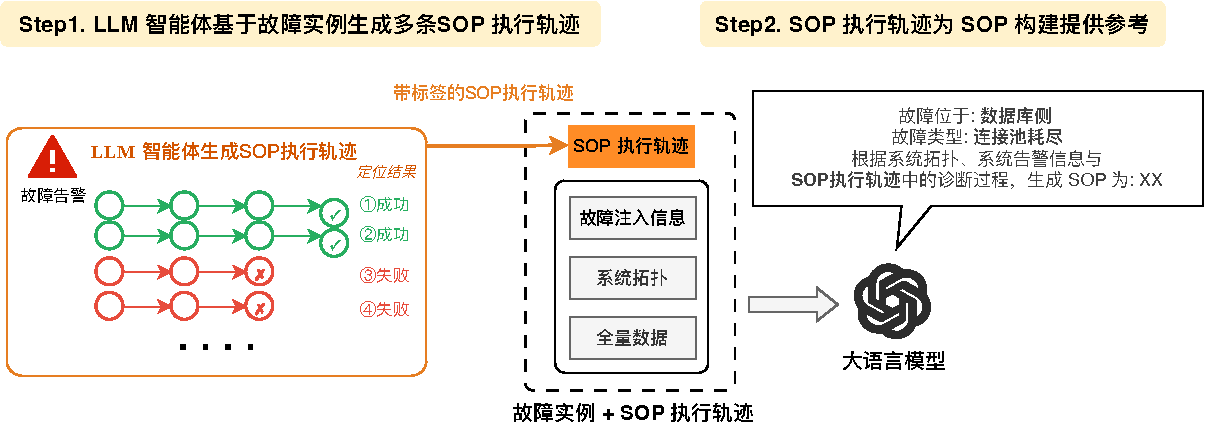
\includegraphics[width=\textwidth]{Figures-Src/Chap3-Methodology/sop-construction-trajectory/chart.pdf}
    \bicaption{\enspace 参照执行轨迹构建SOP的示意}{\enspace Illustration of SOP Construction from Execution Trajectories}
    \label{fig:sop_trajectory_construction}
\end{figure}

为解决仅凭故障观测和最终结论难以直接构建可靠 SOP 的问题，本文在故障实例与最终 SOP 之间引入 \textbf{SOP执行轨迹（SOP Execution Trajectory）} 作为显式中间表示，如图\ref{fig:sop_trajectory_construction}所示。SOP执行轨迹记录离线探索过程中智能体在 SOP 图上的实际执行过程，包括各步检查内容、对应观测证据、路径跳转以及最终诊断结论。因此，SOP 的构建建立在真实执行轨迹之上，而不再依赖模型对中间诊断过程的事后推断。

在引入中间表示之后，还需要进一步确定最终 SOP 的表示形式，使其既能支持后续在线调用，也能支持持续更新。因此面向智能体执行的 SOP 至少应满足以下三项要求：

\begin{enumerate}[label=（\arabic*）]
    \item \textbf{可执行性。} 应显式给出当前需要检查的对象、触发路径转移所依据的证据条件，以及结束排查的判定条件，而不能停留在概括性的自然语言描述上。
    \item \textbf{泛化性。} 不应与某一次故障中的具体服务名、实例名或局部配置直接绑定，否则难以迁移到相似但不完全相同的场景。
    \item \textbf{可增量更新性。} 不应被视为一次性产物，而应能够随着新的执行轨迹持续进行增量更新。
\end{enumerate}

基于上述要求，SOP 不再表示为半结构化的自然语言排障文档，而是借鉴 Think-on-Graph~\cite{sun2024thinkongraph} 中沿图结构逐步推进任务的思路，将 SOP 建模为面向智能体执行的有向无环图（Directed Acyclic Graph，DAG）
\[
G=(V,E),
\]
其中，$V$ 表示诊断节点集合，$E$ 表示节点之间的条件转移关系。Think-on-Graph 将图推理建立在知识图谱中的实体与关系之上，本文则将这一建模思路用于故障诊断流程：图中的节点表示可执行的诊断动作，图中的边表示由观测证据触发的路径转移约束。在线诊断本质上是一个从入口逐步收敛到根因结论的过程。虽然这一过程中可能存在分支选择和路径汇合，但通常不应在既有路径上反复回绕。因此，采用无环结构既有助于智能体稳定执行，也便于后续增量更新。

在该图表示中，节点主要分为入口节点、动作节点和终止节点三类。入口节点对应某类故障排查流程的起点；动作节点表示具体诊断行为，记为
\[
v=\langle \text{Intent}, \text{Entity} \rangle,
\]
其中，$\text{Intent}$ 表示诊断意图，如“检查连接状态”或“验证资源使用率”，$\text{Entity}$ 表示动作作用的目标实体，如“数据库连接池”或“支付服务”；终止节点表示最终识别出的根因结论。边上的条件信息用于刻画节点之间的条件转移关系，即在何种观测结果下进入相应后继节点。基于这种表示，SOP 不再只是对排查流程的静态描述，而成为智能体可直接执行的诊断结构。智能体依据当前观测证据在图上完成判断、执行、观测与转移，并最终收敛到对应的根因结论。


\begin{figure}[!htbp]
    \centering
    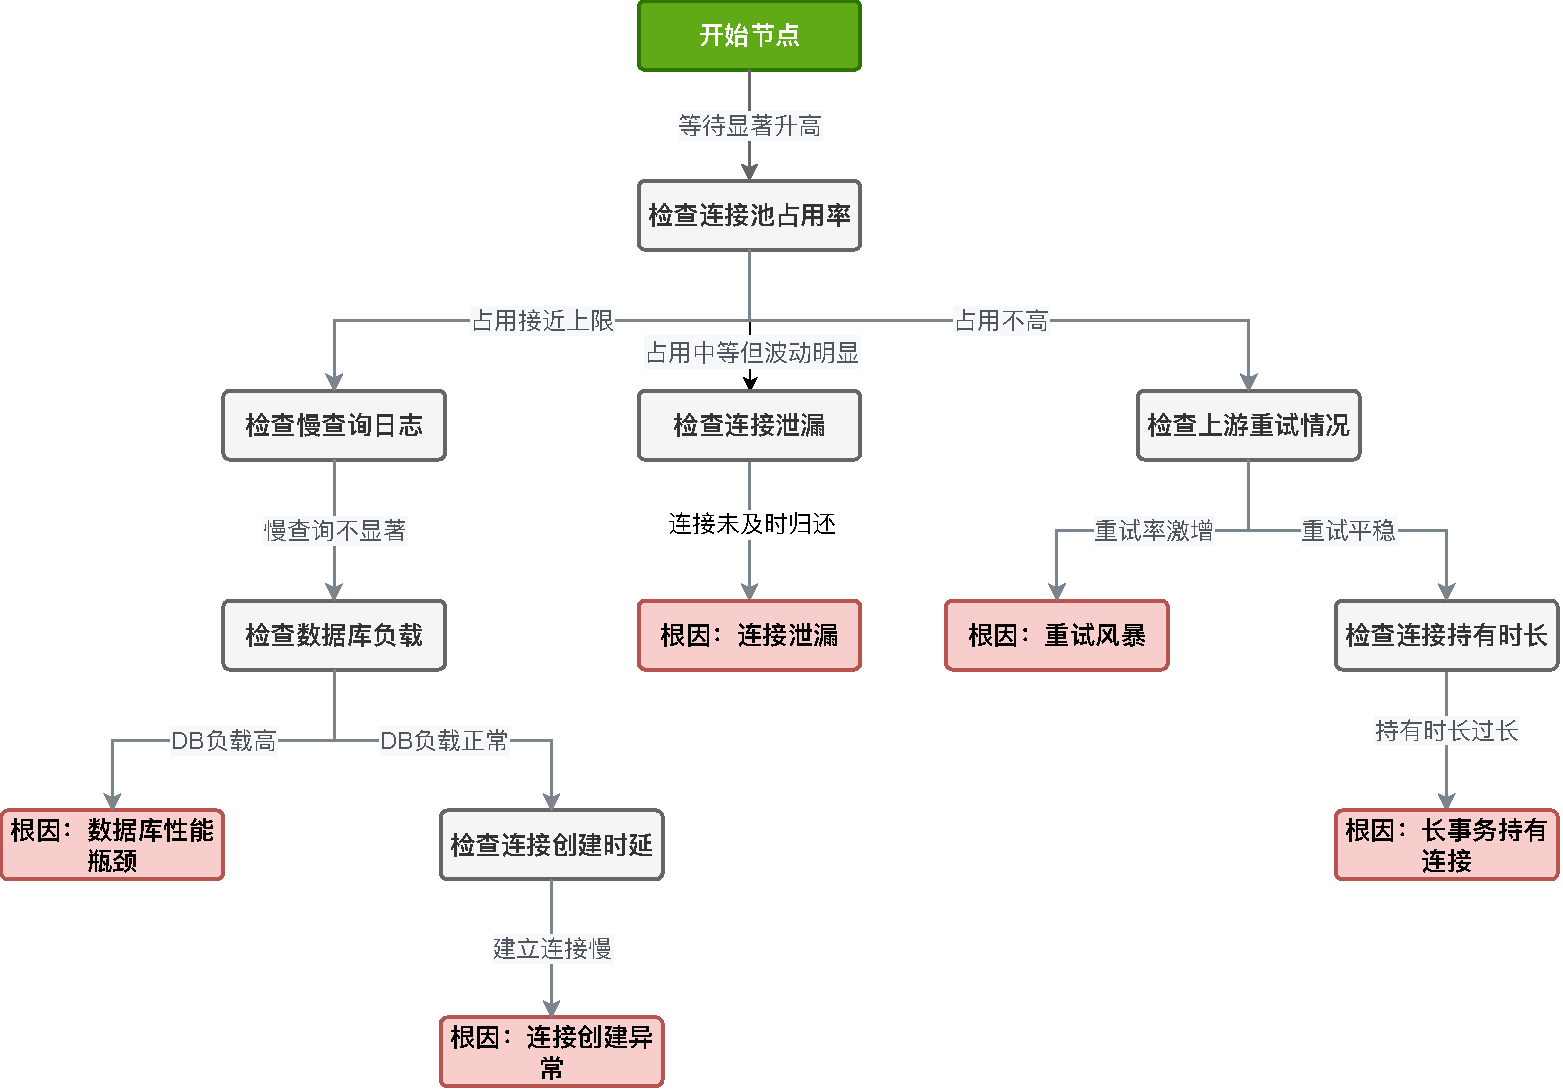
\includegraphics[width=0.75\textwidth]{Figures-Src/Chap3-Methodology/sop-concept-example/chart.pdf}
    \bicaption{\enspace 连接等待显著升高场景的SOP有向无环图示例}{\enspace DAG-based SOP Example for Elevated Connection Wait Time}
    \label{fig:sop_graph_example}
\end{figure}

图\ref{fig:sop_graph_example}给出了数据库场景下的 SOP 有向无环图示例。该图以初始症状为入口，并围绕后续可能的诊断方向组织相应的检查节点。智能体首先检查连接池占用率，再根据“占用接近上限”“占用中等但波动明显”或“占用不高”等不同观测结果，分别进入慢查询日志、连接泄漏、上游重试情况或连接持有时长等后续检查步骤，最终将根因定位为数据库性能瓶颈、连接创建异常、连接泄漏、重试风暴或长事务持有连接等不同结论。该示例说明，SOP 的作用在于将“症状—检查动作—转移条件—根因结论”组织为可执行的诊断流程。

SOP 中的实体不应直接使用历史轨迹中的具体实例名称，而应抽象为可复用的角色化实体。例如，“payment-service-01”应抽象为“上游调用方服务”，“mysql-master-db”应抽象为“数据库连接池组件”。这样既能保留诊断过程中的语义定位信息，又能避免 SOP 绑定于单次实验中的具体实例。至于这些角色化实体如何在在线阶段映射到当前场景中的具体组件，后文将在在线诊断阶段说明。


在此基础上，SOP 的自动化构建可分为三个步骤：

\begin{enumerate}[label=（\arabic*）]
    \item 生成多条 SOP执行轨迹，以显式执行过程还原故障实例中缺失的中间诊断步骤；
    \item 从执行轨迹中提取并对齐决策单元，计算其历史有效性权重；
    \item 在当前版本 SOP 的基础上进行增量整合，形成可执行的有向无环图结构。
\end{enumerate}

经过上述过程，历史故障首先被表示为可比较的诊断执行过程，再进一步整理为可统计、可复用的局部决策结构，最终构造成可直接执行的 SOP 图。

\subsection{故障类型先验的SOP执行轨迹生成}

离线知识构建阶段需要先围绕同一故障实例生成多条可比较的 SOP执行轨迹，用于模拟还原“排查是如何推进的”这一中间过程。本节关注的问题是：\textbf{如何设计离线任务，使智能体能够在历史故障实例上形成可用于后续归纳的诊断执行轨迹。}

一种最直接的做法，是让智能体尽可能模拟真实运维专家的排查方式。具体而言，系统根据故障实例构造模拟的微服务故障环境，智能体只能访问故障窗口内的指标、日志和调用链路等多模态观测数据，并借助相应分析工具逐步缩小可疑范围，最终给出根因结论。系统进一步记录智能体在执行过程中的工具调用与推理过程，作为后续 SOP 构建所需的执行轨迹。由于这种任务设定与真实告警场景最为接近，本文将其称为\textbf{根因定位任务}：智能体不仅需要判断当前故障可能所属的故障类型，还需要继续定位具体的故障组件。

但本文并未直接采用这种任务设定来生成离线轨迹，因为大语言模型在复杂多模态运维数据上的稳定性仍然有限；如果完全以“人类专家视角”独立执行根因定位，智能体往往难以从复杂症状中稳定收敛到真实根因。其直接后果是，正确执行轨迹数量偏少，可用于后续知识沉淀与归纳的正样本不足；而失败轨迹则容易分散到多个无关方向，进一步增加决策单元提取和 SOP 构建的难度。

基于这一考虑，本文将离线任务设定调整为\textbf{故障探索任务}。在该任务中，系统预先给定当前故障的类型标签，探索智能体不再负责判断“这属于哪一类故障”，而是在已知故障类型的前提下，继续围绕该类故障验证可疑组件、传播链路及竞争候选，并记录完整的排查过程。这里引入故障类型先验，并不意味着提前暴露根因位置；其作用在于缩小初始搜索范围，提高有效执行轨迹的比例，并使不同轮次的执行记录能够在同一故障类型内部保持更好的可比性。

设离线故障实例为
\[
\mathcal{I}=(D_{\text{obs}},l^{*},y),
\]
其中，$D_{\text{obs}}$ 表示故障窗口内的可观测数据，$l^{*}$ 表示真实故障位置，$y$ 表示故障类型标签。在轨迹生成阶段，探索智能体可访问的是 $D_{\text{obs}}$、$y$ 和当前版本 SOP $\mathcal{S}$；真实故障位置 $l^{*}$ 对其不可见，仅在轨迹结束后用于判定并标记该轮探索是否成功。

SOP执行轨迹记录的是智能体在 SOP 图上的实际跳转过程。每一步探索都对应一次图上决策：探索智能体根据当前节点、已有证据和故障类型先验判断下一步应检查什么，调用观测能力获取新的指标、日志或调用链路证据，再依据边上的条件决定是否沿现有路径继续推进。若当前 SOP 已经包含足够的节点与边，轨迹就表现为沿既有图结构逐步收敛到根因结论；而在离线构建初期，当前 SOP 往往还是空图，图中既没有可复用节点，也不存在可供满足的出边条件，智能体无法仅依赖现有结构生成轨迹，SOP 结构也难以从空图状态逐步构建。

故障探索任务因此必须允许智能体在必要时扩展图结构。本文将这类操作定义为\textbf{逃逸机制（Escape Mechanism）}。当探索智能体发现当前节点不存在可用出边，或者已有出边的条件与当前证据不匹配，又或者现有 SOP 尚未覆盖当前故障传播路径时，它不再受当前 SOP 已有路径约束，而是依据当前证据自由探索新的诊断方向，并同步构造与这一方向对应的新节点和新边。逃逸本质上是一种在当前 SOP 既有结构之外进行的扩展性探索。它摆脱的是现有路径约束，但探索的目标并不是离开 SOP，而是为 SOP 补入原本尚不存在的节点、边和分支。

在本文设定中，触发逃逸通常对应以下三类情形：

\begin{itemize}
    \item \textbf{当前节点无可用出边。} 现有 SOP 尚未覆盖该状态下的后续诊断动作。
    \item \textbf{已有出边条件与当前证据不匹配。} 现有分支条件不足以解释当前观测，需要构造新的转移关系。
    \item \textbf{需要探索 SOP 尚未覆盖的诊断路径。} 当前故障虽然属于同一类型，但其具体传播方式或可疑对象未被现有 SOP 收录。
\end{itemize}

一次逃逸决策表示为
\[
b_t=\langle v_t^{\mathrm{src}},\rho_t,v_t^{\mathrm{new}},e_t^{\mathrm{new}}\rangle,
\]
其中，$v_t^{\mathrm{src}}$ 表示触发逃逸的源节点，$\rho_t$ 表示触发依据，即当前证据与现有 SOP 不再匹配的原因，$v_t^{\mathrm{new}}$ 表示新建的目标节点，$e_t^{\mathrm{new}}$ 表示连接源节点与目标节点的新边。若该次逃逸最终形成了可验证的根因结论，则说明当前 SOP 在这一类故障下缺少必要的诊断节点、条件边或分支结构；若该次逃逸最终失败，则对应路径只作为失败探索保留在执行轨迹中，而不会直接写入 SOP。一旦某轮探索选择逃逸，后续步骤将沿新生成的路径继续推进；如果在该路径上再次出现“无可用出边”或“条件不匹配”等情形，智能体仍可继续扩展当前逃逸路径。逃逸因此不是一次孤立跳转，而是一条新诊断分支的开始。

故障探索任务由两类智能体协同完成，它们分别负责路径决策和数据观测。

\begin{itemize}
    \item \textbf{探索智能体：} 探索智能体负责在 SOP 图上组织诊断过程。它维护当前节点、已有证据和故障类型先验，决定下一步应检查的对象与诊断意图，并据此选择继续沿现有 SOP 导航、触发逃逸扩展新路径，或在证据满足终止条件时提交根因结论。探索智能体负责基于 SOP 图进行路径决策与过程组织，决定诊断如何推进；而执行过程中实际发生的节点跳转、证据获取和结论提交则会被系统完整记录为 SOP 执行轨迹。
    \item \textbf{观察智能体：} 观察智能体负责与故障实例中的可观测数据交互。它接收探索智能体发送的诊断请求，围绕给定对象与感知域调用指标分析、日志分析和链路查询能力，并将返回结果整理为结构化证据，供探索智能体继续判断。观察智能体不负责决定路径，但它直接决定探索智能体能否获得足够可靠的观测依据。
\end{itemize}


\begin{table}[tbp]
    \centering
    \bicaption{\enspace 探索智能体与观察智能体的工具体系}{\enspace Tool System of the Exploration Agent and Observation Agent}
    \label{tab:dual_agent_tools}
    \renewcommand{\arraystretch}{1.25}
    \fontsize{10pt}{12pt}\selectfont
    \setlength{\tabcolsep}{3pt}
    \begin{tabular*}{\textwidth}{@{\extracolsep{\fill}}>{\centering\arraybackslash}p{1.8cm}>{\centering\arraybackslash}p{2.2cm}>{\raggedright\arraybackslash}p{6.0cm}>{\raggedright\arraybackslash}p{4.0cm}@{}}
        \toprule
        \rowcolor{lightgray!30}
        \textbf{智能体} & \textbf{工具名称} & \textbf{功能描述} & \textbf{关键参数} \\
        \midrule
        \multirow{5}{*}{\textbf{探索智能体}}
        & \texttt{navigate} & 沿 SOP 主链或已有分支跳转 & sop-node-ref \\
        \cline{2-4}
        & \texttt{escape} & 在现有 SOP 无法覆盖时扩展新节点与验证路径 & edge-condition, next-intent \\
        \cline{2-4}
        & \texttt{submit\_message} & 向观察智能体发送查询请求 & prompt \\
        \cline{2-4}
        & \texttt{query\_status} & 查询当前 SOP 状态、节点位置及上下文信息 & current-sop-state \\
        \cline{2-4}
        & \texttt{conclude} & 输出根因结论并汇总关键证据链 & target-component, evidence-chain \\
        \midrule
        \multirow{3}{*}{\textbf{观察智能体}}
        & \texttt{analyze\_metrics} & 当前诊断对象的指标与趋势异常分析 & entity-id \\
        \cline{2-4}
        & \texttt{analyze\_log} & 分析当前诊断对象的日志模式、错误语义及异常事件 & entity-id \\
        \cline{2-4}
        & \texttt{query\_trace} & 查询当前诊断对象的调用链路及上下游 & entity-id \\
        \bottomrule
    \end{tabular*}
    \setlength{\tabcolsep}{6pt}
\end{table}

两类智能体的工具体系如表\ref{tab:dual_agent_tools}所示。探索智能体负责在图上思考、执行跳转、触发逃逸、提交观测请求以及终止任务；观察智能体则负责围绕请求的对象与数据模态，对故障窗口中的指标、日志和调用链路进行具体分析。

在一次故障探索任务中，系统围绕 $(D_{\text{obs}},y,\mathcal{S})$ 重复执行以下过程：探索智能体先根据当前节点、故障类型先验和已有证据确定下一步诊断请求，再通过 \texttt{submit\_message} 将请求发送给观察智能体；观察智能体围绕给定对象调取指标、日志或调用链路证据，并将分析结果返回给探索智能体；探索智能体随后判断应继续沿现有 SOP 图导航，还是触发逃逸扩展新的路径，并在证据充分时提交根因结论。对于执行过程中实际发生的动作、证据获取、节点跳转和结论提交，系统都会统一记录。由此形成的执行记录不仅包含工具调用顺序，也完整保留了智能体在 SOP 图上推进、切换和扩展诊断路径的过程。

系统将第 $r$ 轮探索过程中实际发生的动作、证据、节点跳转、逃逸决策和结论判定统一记录为一条 SOP 执行轨迹，记为
\[
\tau_r=(\mathcal{A}_r,\mathcal{E}_r,\mathcal{P}_r,\mathcal{B}_r,\mathcal{J}_r,\ell_r),
\]
其中，$\mathcal{A}_r$ 表示诊断动作序列，$\mathcal{E}_r$ 表示对应的证据观察，$\mathcal{P}_r$ 表示节点跳转记录，既包括沿现有 SOP 边的导航跳转，也包括由逃逸产生的新边跳转；$\mathcal{B}_r$ 表示逃逸决策记录，其中显式保留源节点、触发依据、新建节点和新建边；$\mathcal{J}_r$ 表示结论判定记录，$\ell_r$ 表示依据真实故障位置 $l^{*}$ 赋予的轨迹标签。

\begin{figure}[tbp]
    \centering
    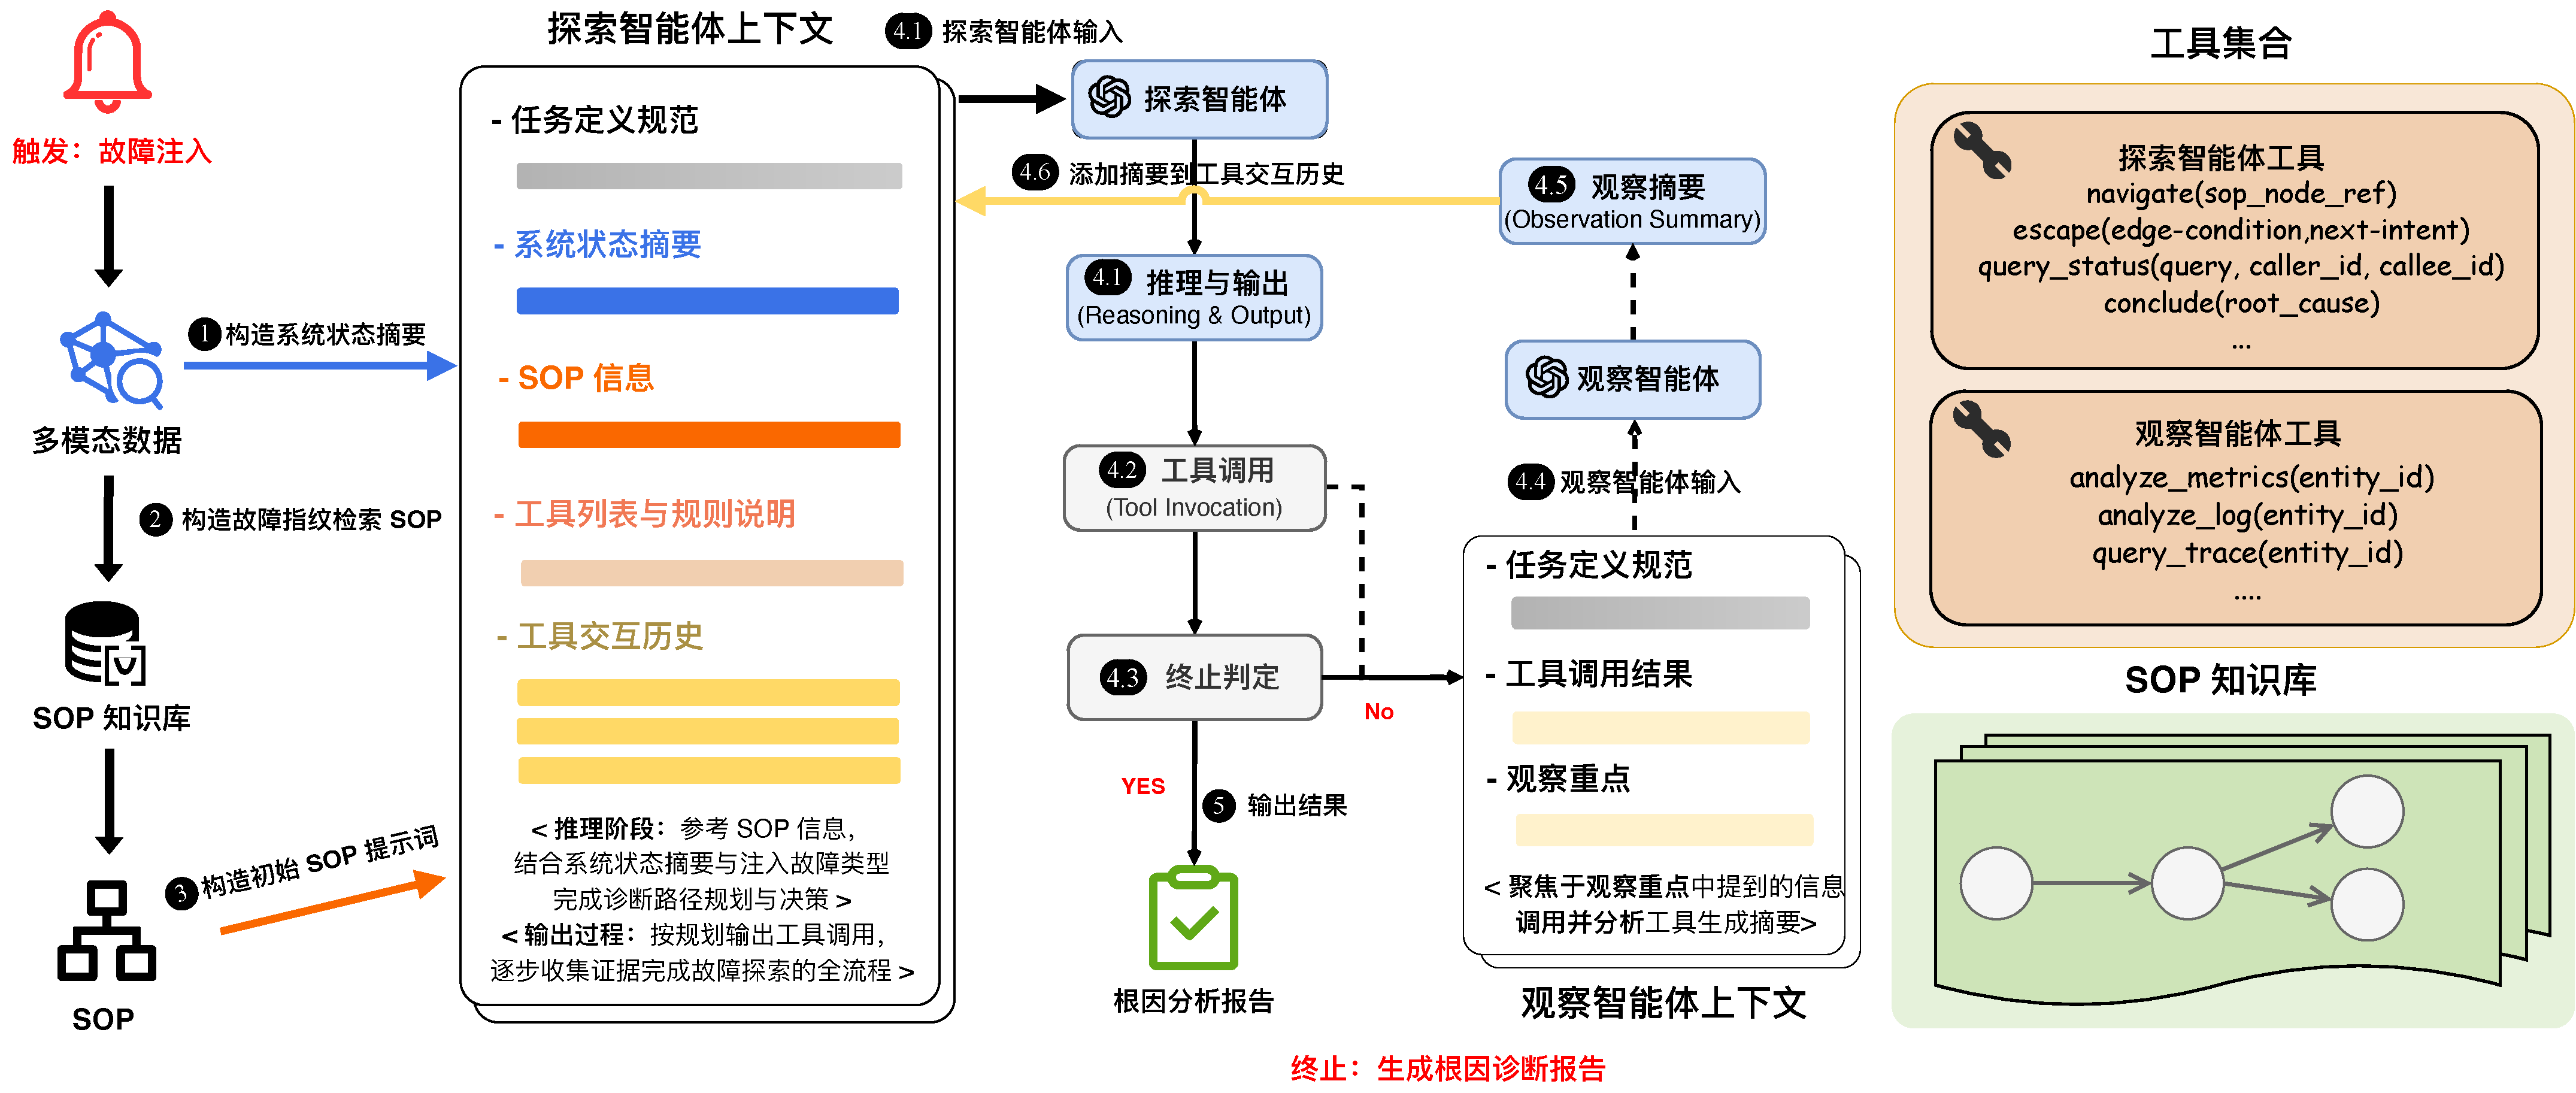
\includegraphics[width=\textwidth]{Figures-Src/Chap3-Methodology/exploration-agent-interaction/chart.pdf}
    \bicaption{\enspace 探索智能体与观察智能体的协作流程}{\enspace Collaboration Flow of the Exploration Agent and Observation Agent}
    \label{fig:exploration_interaction_arch}
\end{figure}

图\ref{fig:exploration_interaction_arch}给出了探索智能体与观察智能体的协作过程。系统提供状态查询、多模态证据分析、导航、逃逸和结论提交五类操作，分别对应 \texttt{query\_status}、\texttt{analyze\_metrics}、\texttt{analyze\_log}、\texttt{query\_trace}、\texttt{navigate}、\texttt{escape} 和 \texttt{conclude}。其中，\texttt{navigate} 对应沿现有 SOP 出边推进，\texttt{escape} 对应在当前图结构无法继续推进时创建新的节点和边。

\begin{figure}[tbp]
    \centering
    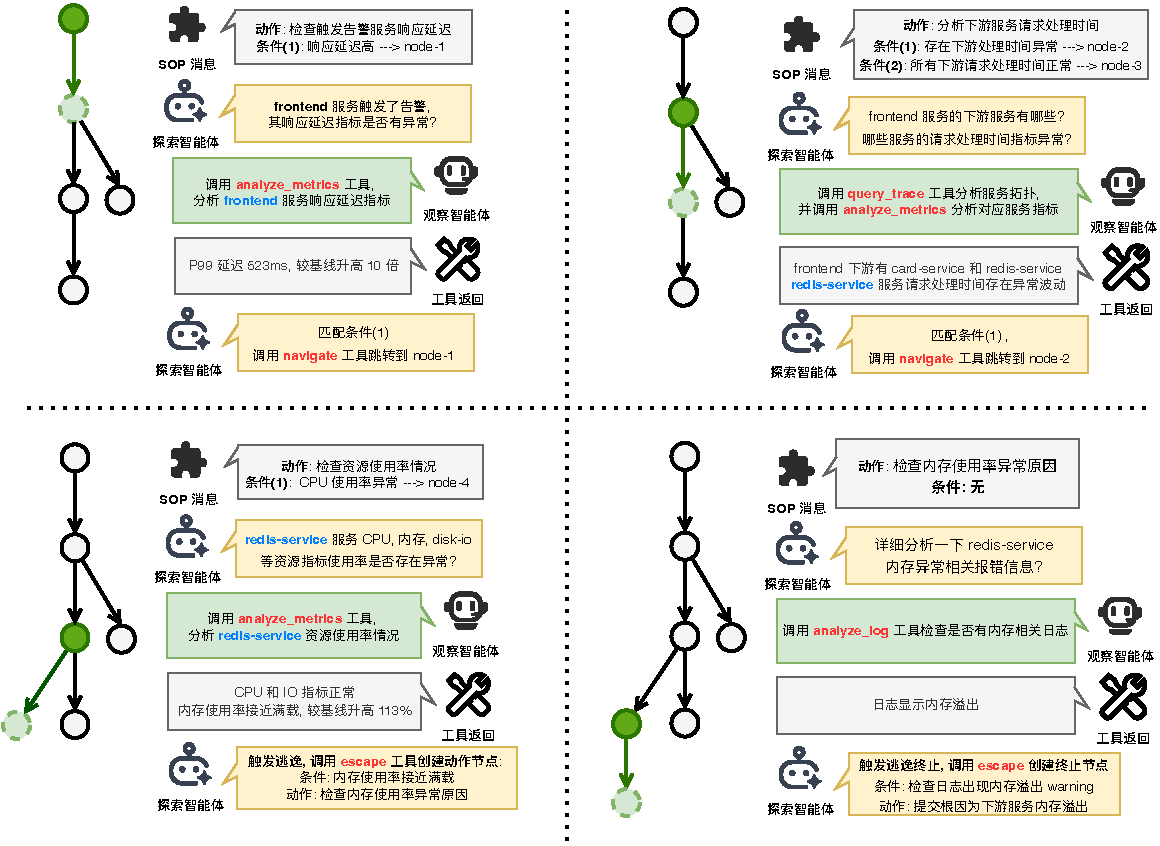
\includegraphics[width=\textwidth]{Figures-Src/Chap3-Methodology/exploration-agent-example/chart.pdf}
    \bicaption{\enspace 探索智能体与观察智能体的协同示例}{\enspace One Collaboration Example of the Exploration Agent and Observation Agent}
    \label{fig:exploration_interaction_example}
\end{figure}

图\ref{fig:exploration_interaction_example}进一步展示了一次具体协同示例：探索智能体根据当前待验证对象调用观察智能体分析指标与日志，并根据返回证据决定继续沿既有路径推进，还是通过逃逸机制生成新的目标节点与转移边。系统以故障实例 $\mathcal{I}=(D_{\text{obs}},l^{*},y)$ 为输入，在当前版本 SOP 的约束下反复执行候选对象初始化、证据收集、路径跳转、逃逸扩展和结论判定等操作。这里的 \texttt{conclude} 仅表示探索智能体提交当前轮次的根因判断，轨迹是否真正成功仍由真实故障位置 $l^{*}$ 在轮次结束后统一标注。

为避免智能体仅凭某个显著异常就过早结束排查，轨迹终止时采用双重结论判定准则：一方面，轨迹中必须形成从表面症状到候选根因的主证据链，即最终结论需要建立在连续、可追溯、能够相互支撑的证据序列之上；另一方面，对于与当前根因判断高度相关的竞争候选，还需要完成排除性验证并给出相应证据。例如，当观察到数据库时延升高时，智能体不能直接将数据库判为根因，还需要进一步排除网络抖动或缓存失效等可能的传播来源。只有当主证据链成立且关键竞争候选被排除后，当前轨迹才被视为满足结论判定条件。

在同一故障场景下，系统会执行多轮相互独立的探索，以获得一组可比较的 SOP执行轨迹。按“是否发生逃逸”和“是否成功定位”两个维度，轨迹被划分为四类：

\begin{enumerate}[label=（\arabic*）]
    \item \textbf{非逃逸成功轨迹。} 现有 SOP 图中已经存在足够的节点、边和条件约束，智能体无需生成新路径即可定位到真实根因，可作为保留主路径的依据。
    \item \textbf{逃逸成功轨迹。} 智能体在某一步找不到可用出边，或现有边条件无法匹配当前证据，因而通过逃逸生成了新的节点和边，并最终成功定位根因。这类轨迹是补全 SOP 新分支的直接来源。
    \item \textbf{非逃逸失败轨迹。} 智能体沿现有主路径推进后仍无法定位根因，表明其中某个条件、节点设计或已有分支结构尚不准确。
    \item \textbf{逃逸失败轨迹。} 智能体虽然生成了新的候选路径，但该路径最终未能形成可验证结论，因此只能作为失败样本保留，而不应直接写入 SOP。
\end{enumerate}

本阶段最终输出的是多条带标签的 SOP 执行轨迹，每条轨迹同时包含动作序列、证据观察、节点跳转、逃逸决策、结论判定以及成败标记。这些轨迹构成后续决策单元提取与权重计算的直接输入；系统同时保留该故障实例对应的故障指纹，用于后续故障簇与 SOP 的绑定。

\subsection{决策单元提取与权重计算}

上一阶段得到的多条 SOP执行轨迹记录了诊断过程中实际发生的检查动作、证据引用、条件转移和阶段性结论，但轨迹本身仍属于过程性记录，尚不能直接纳入 SOP。其原因在于：同一诊断动作在不同轨迹中常以不同表述出现；部分轨迹片段仅对应一次性试探或冗余验证；个别分支虽然被执行，但并未对根因定位产生实质作用。若直接保留整条轨迹，容易使更新后的 SOP 出现节点重复、分支膨胀以及无效步骤混入等问题。

为此，本文先将轨迹拆分为可复用的基本单元，再据此完成后续的 SOP 组织。本文将该基本单元定义为决策单元（Decision Unit），记为
\begin{equation}
u=\langle n,e\rangle,
\end{equation}
其中，节点 $n$ 表示当前诊断动作，
\begin{equation}
n=\langle \text{Intent},\text{Entity}\rangle,
\end{equation}
边 $e$ 表示由条件触发的转移关系，
\begin{equation}
e=\langle \text{Condition},\text{Next}\rangle.
\end{equation}
其中，$\text{Intent}$ 表示当前步骤的检查意图，$\text{Entity}$ 表示被检查对象，$\text{Condition}$ 表示触发转移的判断条件，$\text{Next}$ 表示满足条件后的后继节点。这样，一个决策单元同时刻画了“当前检查什么”以及“在何种条件下转向何处”两个信息。例如，“检查数据库连接池状态”与“若连接数达到上限，则转向检查连接泄漏”可共同表示为一个完整的决策单元。

设 SOP执行轨迹集合为 $\mathcal{T}=\{\tau_1,\tau_2,\ldots,\tau_N\}$，则每条轨迹首先被拆分为决策单元序列
\begin{equation}
\mathcal{U}_{\tau_i}=\textsc{SplitUnits}(\tau_i),
\end{equation}
并汇总得到候选决策单元集合
\begin{equation}
\mathcal{U}=\bigcup_{i=1}^{N}\mathcal{U}_{\tau_i}.
\end{equation}
这里，$\mathcal{U}$ 同时包含沿既有 SOP 路径抽取的决策单元，以及由逃逸机制生成并在后续执行中被验证的新增决策单元。

为消除表述差异带来的重复记载，本文将每个决策单元统一编码为文本序列
\begin{equation}
c(u)=\text{Intent}\oplus \text{Entity}\oplus \text{Condition},
\end{equation}
并利用语义嵌入模型将其映射到向量空间
\begin{equation}
\mathbf{z}_{u}=f_{\mathrm{emb}}\big(c(u)\big).
\end{equation}
在此基础上，对向量集合 $\{\mathbf{z}_{u}\mid u\in\mathcal{U}\}$ 进行基于密度的聚类，得到语义一致的决策单元簇
\begin{equation}
\mathcal{C}=\{C_{1},C_{2},\ldots,C_{M}\}=\textsc{DBSCAN}\big(\{\mathbf{z}_{u}\}\big).
\end{equation}
每个簇 $C_j$ 对应一类语义相近、但原始表述可能不同的决策单元。

完成语义对齐后，本文进一步从历史轨迹中评估各决策单元簇的保留价值。考虑到 SOP 更新的目标是保留能够稳定支持根因定位的步骤，本文从互信息、方向性、拓扑位置和逃逸有效性四个维度对每个簇 $C_j$ 进行加权。

\paragraph{1) 互信息（Mutual Information, MI）}
互信息用于度量决策单元簇 $C_j$ 与诊断成功之间的统计关联。设
\begin{equation}
x_{\tau,j}=\mathbb{I}(C_j \cap \mathcal{U}_{\tau}\neq \varnothing),
\end{equation}
表示轨迹 $\tau$ 中是否出现过簇 $C_j$，$y_{\tau}\in\{0,1\}$ 表示该轨迹是否成功定位根因，则
\begin{equation}
\mathrm{MI}_{j}=\sum_{x\in\{0,1\}}\sum_{y\in\{0,1\}}p_{j}(x,y)\log \frac{p_{j}(x,y)}{p_{j}(x)\,p(y)}.
\end{equation}
$\mathrm{MI}_{j}$ 越大，说明该决策单元与成功诊断的关联越强，更适合作为稳定步骤写入 SOP。

\paragraph{2) 方向因子（Direction Factor, DF）}
方向因子用于衡量某一决策单元在执行后是使诊断更接近根因，还是使路径偏离主线。记 $O_j$ 为簇 $C_j$ 在全部轨迹中的出现位置集合。对于任一出现位置 $(\tau,t)\in O_j$，设 $d^-_{\tau,t}$ 表示执行该单元之前当前节点到终止节点的剩余步数，$d^+_{\tau,t}$ 表示执行该单元并完成转移后到终止节点的剩余步数，则
\begin{equation}
\mathrm{DF}_{j}=\frac{1}{|O_j|}\sum_{(\tau,t)\in O_j}\frac{d^-_{\tau,t}-d^+_{\tau,t}}{d^-_{\tau,t}+1}.
\end{equation}
当 $\mathrm{DF}_{j}>0$ 时，说明该决策单元总体上推动路径朝终止节点收敛；当 $\mathrm{DF}_{j}<0$ 时，说明该单元更常出现在偏离根因的路径中。

\paragraph{3) 拓扑距离（Topology Distance, TD）}
拓扑距离用于描述决策单元在一条有效诊断路径中的相对位置。对于出现位置 $(\tau,t)\in O_j$，设 $L_{\tau}$ 为轨迹 $\tau$ 的总步数，$\ell_{\tau,t}$ 为该位置到轨迹终止节点的剩余步数，则定义
\begin{equation}
\mathrm{TD}_{j}=1-\frac{1}{|O_j|}\sum_{(\tau,t)\in O_j}\frac{\ell_{\tau,t}}{L_{\tau}}.
\end{equation}
$\mathrm{TD}_{j}$ 越大，说明该决策单元越接近诊断收敛位置。该指标可用于区分早期的广泛筛查步骤与后期具有更强定位作用的关键步骤。

\paragraph{4) 逃逸有效性（Escape Validity, EV）}
逃逸有效性用于衡量决策单元在逃逸路径中的实际贡献。记 $O_j^{\mathrm{esc}}\subseteq O_j$ 为簇 $C_j$ 在逃逸路径中的全部出现位置集合，则
\begin{equation}
\mathrm{EV}_{j}=
\frac{\sum_{(\tau,t)\in O_j^{\mathrm{esc}}} y_{\tau}}
{|O_j^{\mathrm{esc}}|+\varepsilon},
\end{equation}
其中，$\varepsilon$ 为防止分母为零的平滑项。当 $\mathrm{EV}_{j}$ 较高时，说明该决策单元虽然并非总来自既有 SOP 主路径，但在历史逃逸过程中多次参与了有效收敛，因而具有保留价值。

由于四个指标的量纲不同，本文先对各指标进行归一化处理。对于任一指标 $s\in\{\mathrm{MI},\mathrm{DF},\mathrm{TD},\mathrm{EV}\}$，记其归一化结果为
\begin{equation}
\widehat{s}_{j}=
\frac{s_{j}-\min_{k}s_{k}}
{\max_{k}s_{k}-\min_{k}s_{k}+\varepsilon}.
\end{equation}
在此基础上，决策单元簇 $C_j$ 的综合权重定义为
\begin{equation}
w_j=\alpha_{1}\widehat{\mathrm{MI}}_{j}
+\alpha_{2}\widehat{\mathrm{DF}}_{j}
+\alpha_{3}\widehat{\mathrm{TD}}_{j}
+\alpha_{4}\widehat{\mathrm{EV}}_{j},
\qquad
\sum_{m=1}^{4}\alpha_m=1.
\end{equation}
其中，$\alpha_m$ 为各指标的组合系数。$w_j$ 并不直接决定某一决策单元是否被保留，而是为后续 SOP 增量更新提供排序依据：当多个候选步骤具有相似语义时，权重更高者优先进入 SOP 结构。

综上，经过拆分、对齐与加权后，系统得到带权决策单元集合
\begin{equation}
\mathcal{U}^{w}=\{u^{w}_{1},u^{w}_{2},\ldots,u^{w}_{M}\}.
\end{equation}
集合中的每个元素均包含统一语义标识、诊断意图、目标实体、触发条件及其综合权重。相较于原始轨迹，带权决策单元已经从过程性记录转化为可直接参与 SOP 更新的结构化知识，可作为后续 SOP 增量组织与更新的直接输入。

\begin{algorithm}[!t]
    \caption{\enspace 决策单元提取、对齐与加权算法}
    \label{alg:decision_unit_weighting}
    \begin{algorithmic}[1]
        \Require SOP执行轨迹集合 $\mathcal{T}$，轨迹标签集合 $\mathcal{Y}$，语义嵌入模型 $f_{\mathrm{emb}}$，组合系数向量 $\boldsymbol{\alpha}=(\alpha_1,\alpha_2,\alpha_3,\alpha_4)$
        \Ensure 带权决策单元集合 $\mathcal{U}^{w}$
        
        \State 初始化候选决策单元集合 $\mathcal{U}\leftarrow \varnothing$
        \State 初始化带权决策单元集合 $\mathcal{U}^{w}\leftarrow \varnothing$
        
        \ForAll{轨迹 $\tau \in \mathcal{T}$}
            \State $\mathcal{U}_{\tau}\leftarrow \textsc{SplitUnits}(\tau)$ \Comment{从轨迹中切分决策单元}
            \State $\mathcal{U}\leftarrow \mathcal{U}\cup \mathcal{U}_{\tau}$
        \EndFor
        
        \ForAll{$u\in \mathcal{U}$}
            \State $c(u)\leftarrow \textsc{Serialize}(u)$ \Comment{序列化为统一文本表示}
            \State $\mathbf{z}_{u}\leftarrow f_{\mathrm{emb}}(c(u))$ \Comment{计算语义嵌入表示}
        \EndFor
        
        \State $\mathcal{C}\leftarrow \textsc{DBSCAN}(\{\mathbf{z}_{u}\mid u\in\mathcal{U}\})$ \Comment{聚类得到语义对齐后的决策单元簇}
        
        \ForAll{决策单元簇 $C_j\in\mathcal{C}$}
            \State $(\mathrm{MI}_{j},\mathrm{DF}_{j},\mathrm{TD}_{j},\mathrm{EV}_{j})\leftarrow \textsc{EstimateScores}(C_j,\mathcal{T},\mathcal{Y})$
            \State $\mathbf{s}_{j}\leftarrow (\mathrm{MI}_{j},\mathrm{DF}_{j},\mathrm{TD}_{j},\mathrm{EV}_{j})$
            \State $\widehat{\mathbf{s}}_{j}\leftarrow \textsc{Normalize}(\mathbf{s}_{j})$ \Comment{对四类评分进行归一化}
            \State $w_{j}\leftarrow \sum_{m=1}^{4}\alpha_{m}\widehat{s}_{j,m}$ \Comment{计算簇级权重}
            \State $u_{j}^{w}\leftarrow \textsc{AggregateUnit}(C_j,w_j)$ \Comment{生成带权代表性决策单元}
            \State $\mathcal{U}^{w}\leftarrow \mathcal{U}^{w}\cup\{u_{j}^{w}\}$
        \EndFor
        
        \State \Return $\mathcal{U}^{w}$
    \end{algorithmic}
\end{algorithm}


\subsection{规则智能体的SOP组织方法}

带权决策单元（Decision Unit）给出了“哪些局部判断值得保留”的统计结果，但最终更新至系统的不是若干彼此分散的决策单元，而是一份能够被在线诊断直接执行的 SOP。RuleAgent 的工作，就是把这些决策单元重新放回到完整的诊断路径中，判断它们应该被加在什么位置、删掉什么旧步骤、以及修改哪些已有条件。

RuleAgent 的输入包括三部分：当前版本 SOP、该故障实例下的全部 SOP执行轨迹，以及带权决策单元库。按照前文定义，输入的 SOP执行轨迹已经依据“是否发生逃逸”和“是否成功收敛到根因”完成四类标签标记。这样，RuleAgent 在观察一条路径时，不仅知道某个步骤是否出现过，还知道它更常出现在何种结果的路径中：是推动诊断收敛，还是把诊断带向无效分支。带权决策单元库则提供局部判断的历史统计结果，用于区分“反复有效的步骤”和“偶然出现的动作”。

RuleAgent 不直接根据轨迹生成一份全新的 SOP，而是围绕当前版本 SOP 做局部更新。新的故障实例会暴露出结构缺口、低价值路径或条件表达不准确等问题；同类故障反复出现时，RuleAgent 再在上一版本的基础上补全、收缩或改写相关结构。提示词模板要求 RuleAgent 先对照当前 SOP 查找轨迹片段对应的位置，再结合轨迹标签和决策单元权重判断该片段应被视为新增步骤、无效步骤还是条件改写线索。

\begin{figure}[!htbp]
    \centering
    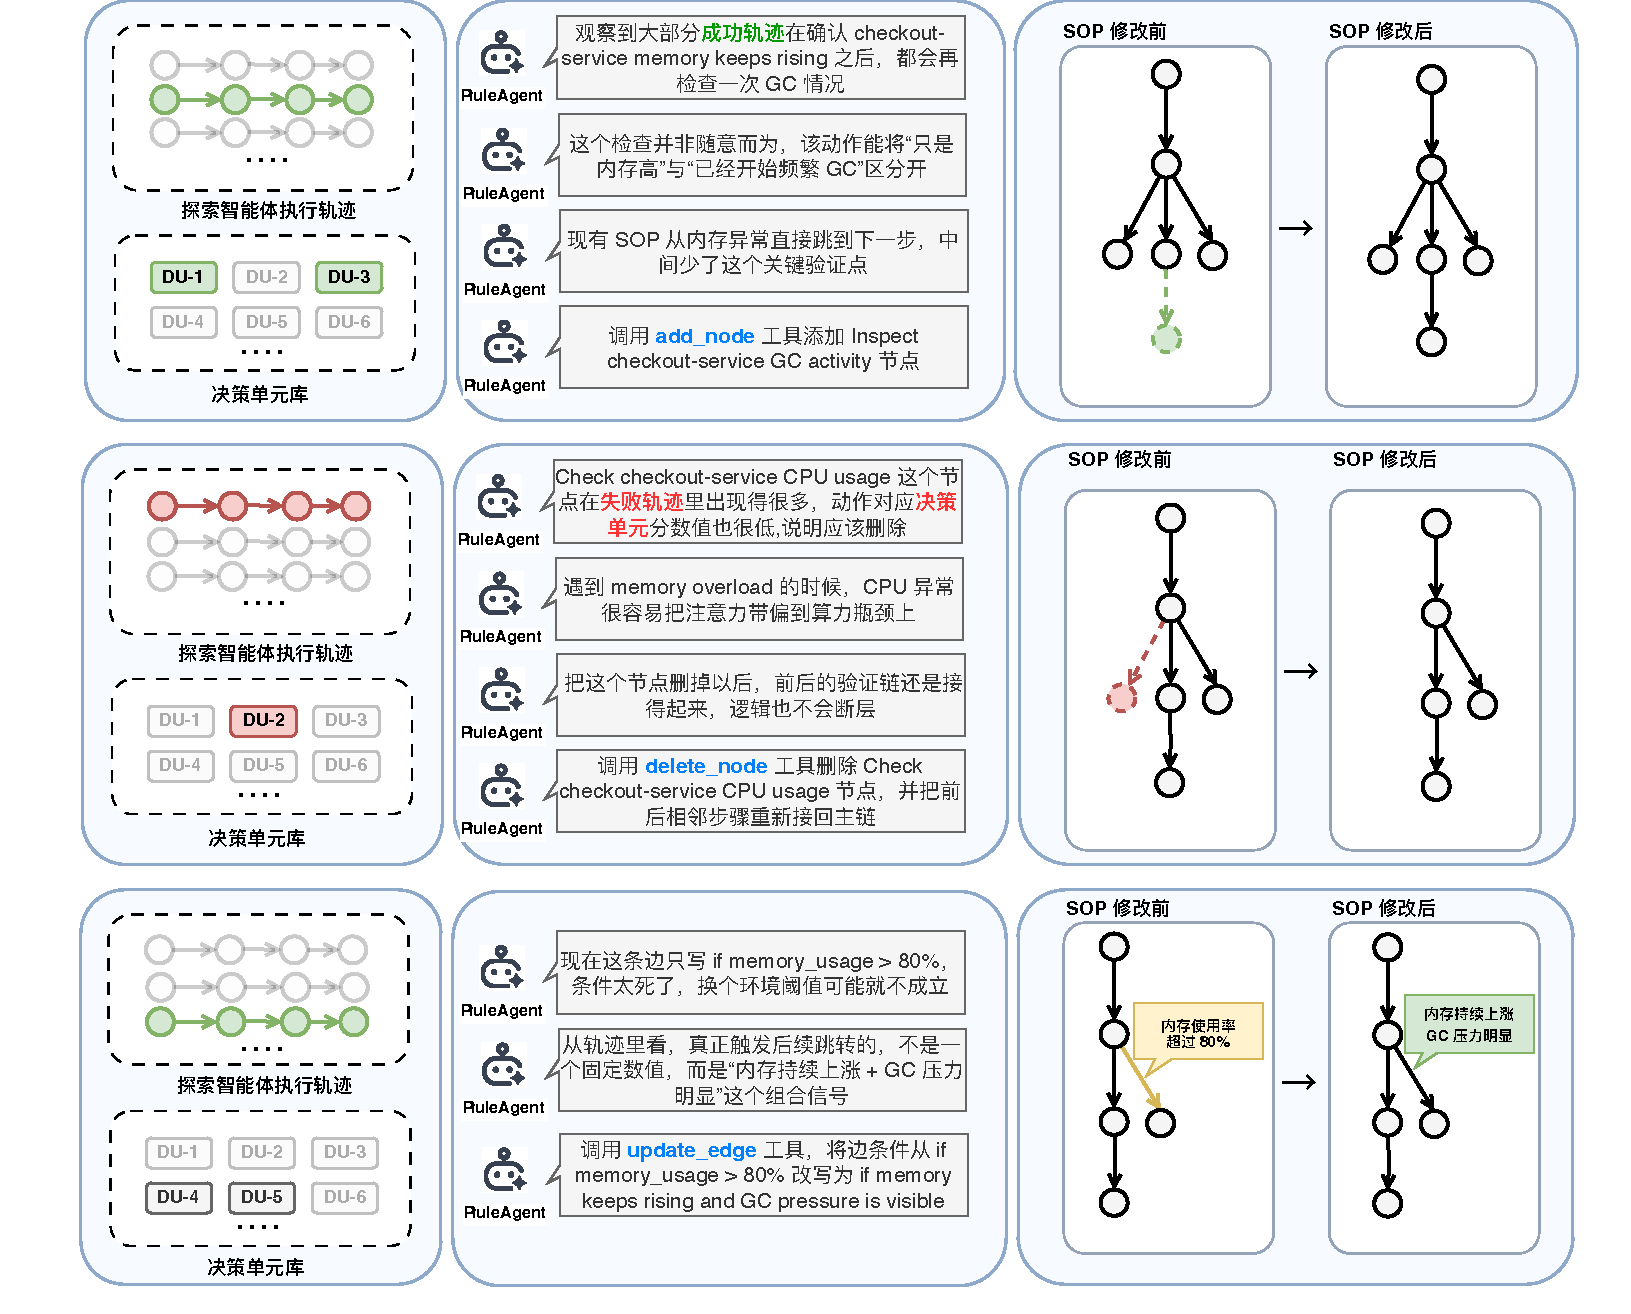
\includegraphics[width=\textwidth]{Figures-Src/Chap3-Methodology/sop-construction-case/chart.pdf}
    \bicaption{\enspace 执行轨迹构建SOP的示意}{\enspace Illustration of SOP Construction from Execution Trajectories}
    \label{fig:sop_rule}
\end{figure}

结合图\ref{fig:sop_rule}，RuleAgent 对 SOP 的组织主要体现在三类操作上：添加、删除和修改。

\begin{enumerate}[label=（\arabic*）]
    \item \textbf{添加：把当前 SOP 中缺失、但已被多次验证有效的检查步骤补入原有路径。}图\ref{fig:sop_rule}上半部分给出了一个新增节点的例子。多条成功轨迹表明，在确认 \texttt{checkout-service} 内存持续升高之后，诊断过程通常还会继续检查一次 GC 状态；而现有 SOP 在“内存异常”之后直接跳转到下一步，中间缺少这一检查节点。RuleAgent 在对照轨迹时，会先从当前 SOP 中定位到“内存异常”所在节点，再结合带权决策单元库判断“检查 GC 情况”是否属于反复出现且有效的局部判断。若答案为是，则调用 \texttt{add\_node} 与 \texttt{add\_edge}，把 \texttt{Inspect checkout-service GC activity} 作为新的中间节点插入原路径中。新增的不是一条临时轨迹片段，而是一个已经被多次成功执行支持的缺失步骤。

    \item \textbf{删除：把长期误导诊断、且在失败路径中频繁出现的步骤从 SOP 中移除。}图\ref{fig:sop_rule}中间部分展示了一个删除节点的例子。节点“\texttt{Check checkout-service CPU usage}”在失败轨迹中出现频繁，而对应决策单元的权重也较低，说明该检查步骤虽然经常被执行，但并没有稳定帮助诊断收敛。在内存过载场景下，这一步往往把排查方向过早引向 CPU 瓶颈，造成注意力偏移。RuleAgent 在读取全部已标记轨迹后，会发现该节点更多出现在未能收敛的路径中，并且删除该节点后，前后的验证关系仍然可以自然衔接。因此，它会调用 \texttt{delete\_node} 或 \texttt{delete\_edge}，将这一低价值步骤从当前 SOP 中移除，并把前后相邻节点重新接回主链。删除的依据不是“这一步出现次数少”，而是“这一步反复出现，但对正确定位根因没有形成稳定贡献”。

    \item \textbf{修改：保留原有节点或边，但把过于僵硬或不准确的表达改写为更符合真实诊断规律的条件。}图\ref{fig:sop_rule}下半部分对应的是条件修改。旧版本 SOP 只写“\texttt{if memory\_usage > 80\%}”，这类固定阈值便于书写，但与真实诊断过程并不完全一致。轨迹显示，真正触发后续排查的并不是某个孤立的数值点，而是“内存持续上升，同时伴随明显 GC 压力”的组合信号。RuleAgent 在比较多条执行轨迹后，会发现当“内存持续升高 + GC 压力明显”出现时，后续路径具有更高的一致性，而单独的“超过 80\%”并不能稳定区分是否需要继续下钻。因此，它不会删除该分支，而是调用 \texttt{update\_edge}，把原来的边条件改写为更贴近真实触发模式的表达。修改保留了原有结构，但提升了 SOP 条件语义的准确性。
\end{enumerate}

这三类操作分别对应补足缺失步骤、清理误导路径和修正触发条件。随着同类故障实例不断积累，这些局部更新会反复发生，因此 SOP 的形成本质上是一个持续校正和逐步补全的过程。

为了使上述编辑可追踪、可回滚，RuleAgent 的行为被限制在一组智能体工具之内。表\ref{tab:ruleagent_tools}给出了 RuleAgent 在组织 SOP 时使用的工具集合。

\begin{table}[tbp]
    \centering
    \bicaption{\enspace 规则智能体的 SOP 组织工具}{\enspace Tools Used by RuleAgent for SOP Organization}
    \label{tab:ruleagent_tools}
    \renewcommand{\arraystretch}{1.25}
    \fontsize{10pt}{12pt}\selectfont
    \setlength{\tabcolsep}{3pt}
    \begin{tabular*}{\textwidth}{@{\extracolsep{\fill}}>{\centering\arraybackslash}p{2.0cm}>{\centering\arraybackslash}p{1.9cm}>{\raggedright\arraybackslash}p{5.2cm}>{\raggedright\arraybackslash}p{4.0cm}@{}}
        \toprule
        \rowcolor{lightgray!30}
        \textbf{工具类别} & \textbf{工具名称} & \textbf{功能描述} & \textbf{关键参数} \\
        \midrule
        \multirow{3}{*}{\textbf{知识读取}}
        & \texttt{get\_decision\_unit} & 读取当前故障类型的带权决策单元及统计信息 & fault-type \\
        \cline{2-4}
        & \texttt{read\_trajectory} & 读取当前故障类型的已标记执行轨迹及上下文证据 & fault-type, label, batch-size \\
        \cline{2-4}
        & \texttt{read\_sop} & 读取当前版本 SOP 的节点、边及版本信息 & sop-id, version \\
        \midrule
        \multirow{7}{*}{\textbf{SOP 局部更新}}
        & \texttt{add\_node} & 插入新的诊断动作节点 & parent-node-id, intent, entity \\
        \cline{2-4}
        & \texttt{add\_edge} & 添加条件跳转关系 & source-node-id, target-node-id, condition \\
        \cline{2-4}
        & \texttt{update\_node} & 更新节点意图或实体表达 & node-id, intent, entity \\
        \cline{2-4}
        & \texttt{update\_edge} & 更新边条件或约束语义 & edge-id, condition \\
        \cline{2-4}
        & \texttt{delete\_node} & 删除无效或重复节点 & node-id \\
        \cline{2-4}
        & \texttt{delete\_edge} & 删除无效跳转关系 & edge-id \\
        \cline{2-4}
        & \texttt{save\_sop} & 保存 SOP 版本及更新说明 & sop-id, version-note \\
        \bottomrule
    \end{tabular*}
    \setlength{\tabcolsep}{6pt}
\end{table}

经过上述组织后，系统得到的不是脱离旧版本重新生成的一张新图，而是在当前版本 SOP 上完成的一次局部更新结果。一次故障实例可能只暴露出一个缺失节点，也可能只说明某条旧路径应被删除，或者只推动某个条件表达被改写；当同类故障不断出现时，这些局部写回会持续累积到同一份 SOP 上，使其中的诊断知识被一步一步提取出来。最终得到的 SOP 仍表示为有向无环图，并与对应故障簇建立绑定关系，供后续在线诊断阶段直接召回与执行。


%---------------------------------------------------------------------------%
%->> 3.4 SOP驱动的多智能体在线故障诊断方法
%---------------------------------------------------------------------------%
%---------------------------------------------------------------------------%
%->> Section 3.4: SOP驱动的多智能体在线故障诊断方法
%---------------------------------------------------------------------------%

\section{SOP驱动的多智能体在线故障诊断方法}

\begin{figure}[htbp]
    \centering
    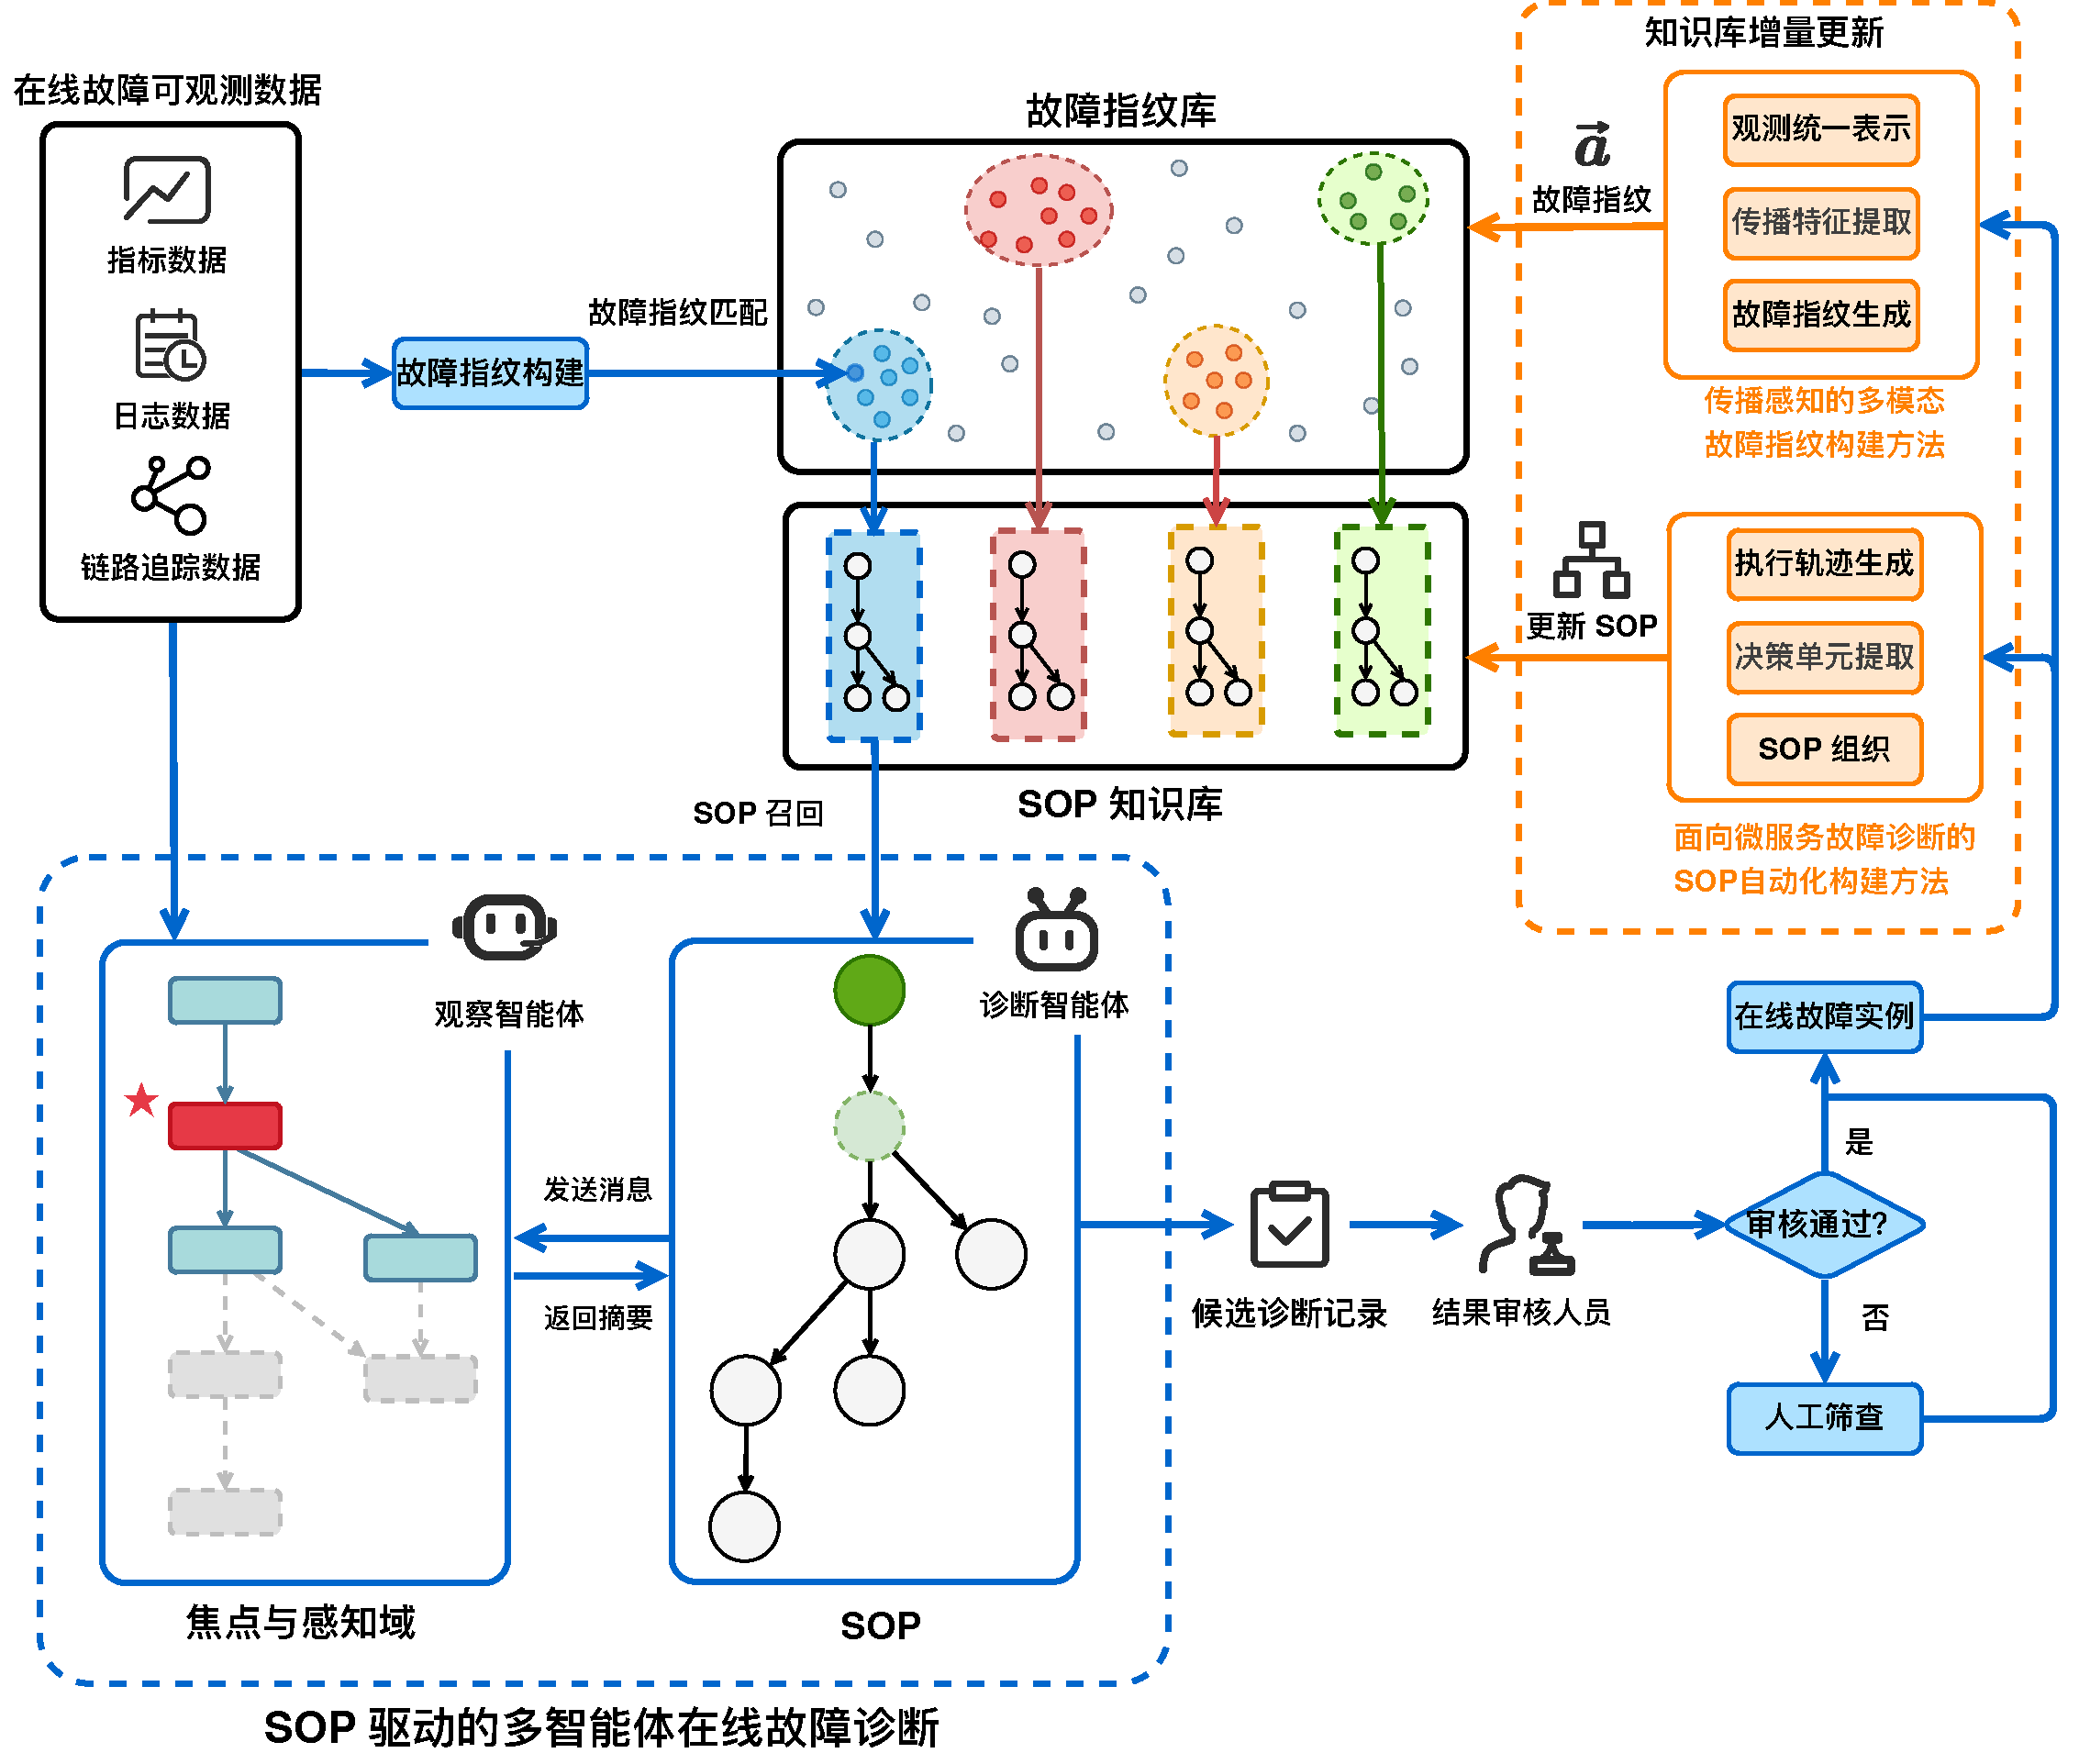
\includegraphics[width=0.8\textwidth]{Figures-Src/Chap3-Methodology/online-diagnosis-overview/chart.pdf}
    \bicaption{\enspace SOP驱动的多智能体在线故障诊断总览}{\enspace Overview of SOP-Driven Multi-Agent Online Fault Diagnosis}
    \label{fig:online_diagnosis_overview}
\end{figure}

图\ref{fig:online_diagnosis_overview}给出了SOP驱动的多智能体在线故障诊断总览。在线阶段以上两节构建的故障指纹库和 SOP 知识库为基础：当生产环境中出现新故障时，系统先根据当前故障的指标、日志和调用链路数据生成故障指纹，并在故障指纹库中检索最相似的历史故障簇，召回其绑定的 SOP 作为初始排查路径。随后，诊断智能体与观察智能体协同执行在线诊断。诊断结束后，结果经人工审核确认，作为新的在线故障实例重新进入第3.2节和第3.3节的知识构建流程。

本节其余内容按上述流程展开：3.4.1节介绍故障指纹生成与SOP召回；3.4.2节介绍焦点与感知域约束；3.4.3节介绍SOP驱动的多智能体在线诊断流程；3.4.4节介绍在线诊断结果审核与SOP增量更新。

\subsection{故障指纹匹配与 SOP 召回}

离线阶段中，系统首先按照第3.2节的方法为每个故障实例生成故障指纹向量，并在此基础上对相似故障实例进行聚类；随后，再按照第3.3节的方法为每个故障簇维护与其对应的可执行SOP。在线阶段不能将当前故障直接对应到某一条离线SOP，因为线上故障通常只与某一类历史故障相近，而不会与某个离线故障实例在服务实例、传播范围和局部现象上完全一致。例如，历史故障可能表现为“支付服务的数据库连接池耗尽”，而当前故障则可能表现为“订单服务的数据库连接池耗尽”。二者虽然属于同类故障，但涉及的组件实例和传播路径并不相同；若直接匹配单个历史故障实例，就容易将某次离线试验中的局部细节误当作当前场景中的通用排查路径，从而影响SOP的可执行性。因此，本文将SOP绑定到故障簇，而不是绑定到某个单独的故障实例，如图\ref{fig:fingerprint_sop_binding}所示。采用按故障簇召回SOP的方式，可以保留同类故障中稳定出现的排查步骤，减弱个别实例差异对在线诊断的影响。

\begin{figure}[htbp]
    \centering
    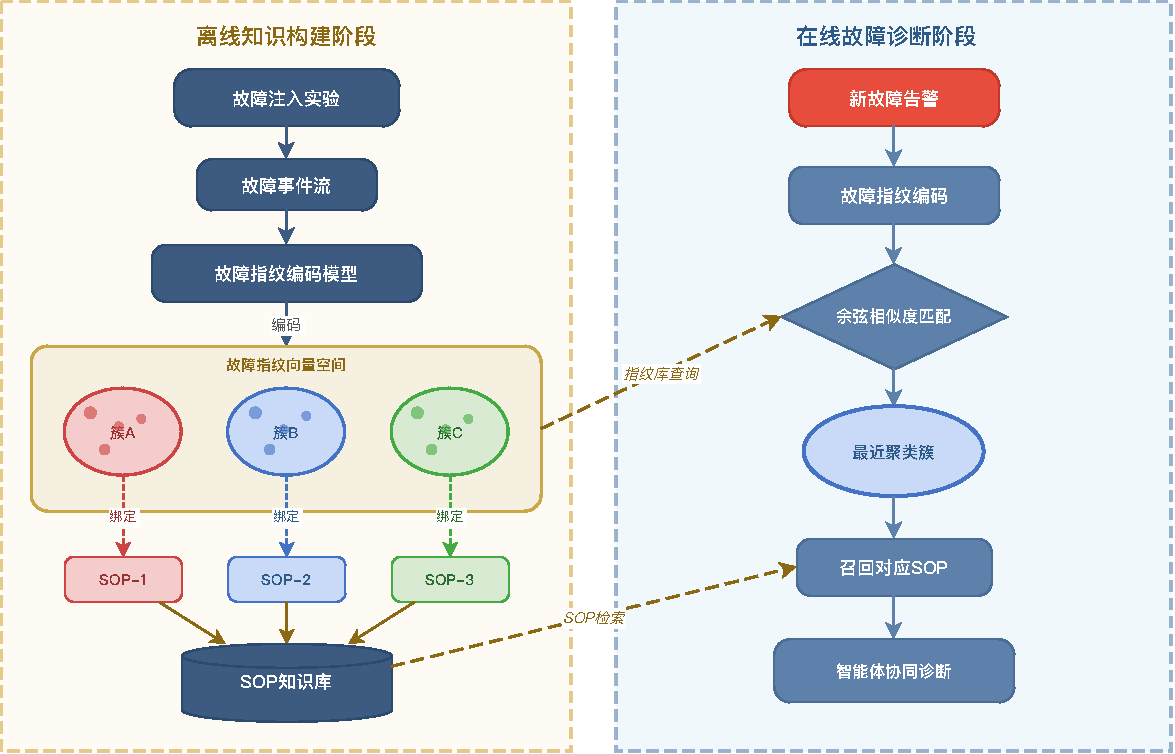
\includegraphics[width=\textwidth]{Figures-Src/Chap3-Methodology/fingerprint-sop-binding/chart.pdf}
    \bicaption{\enspace 故障指纹聚类、SOP绑定与在线召回}{\enspace Fault Fingerprint Clustering, SOP Binding, and Online Recall}
    \label{fig:fingerprint_sop_binding}
\end{figure}

对于每个故障簇，系统保存其中心向量 $\mathbf{c}_i$ 及对应的SOP。在线阶段接收新故障告警后，首先从当前故障的可观测数据中提取异常事件，并通过第3.2节中的故障指纹构建方法生成当前故障向量 $\mathbf{v}_{\text{fault}}$；随后，计算该向量与各故障簇中心向量之间的余弦相似度，并选择最相似的故障簇所绑定的SOP作为当前故障的初始排查路径：
\begin{equation}
\text{SOP}_{\text{selected}}=\arg\max_i \frac{\mathbf{v}_{\text{fault}}\cdot \mathbf{c}_i}{\|\mathbf{v}_{\text{fault}}\|\|\mathbf{c}_i\|}.
\end{equation}

完成SOP召回后，系统将诊断智能体初始化至 $\text{SOP}_{\text{selected}}$ 的入口节点，使其能够从召回的排查起点开始组织后续诊断过程。至此，系统完成了从当前故障观测数据到初始 SOP 的映射，并为后续受约束在线诊断提供了流程基础。

\subsection{焦点与感知域约束}

在前文第3.3节介绍的探索智能体基于 SOP 的探索任务执行中，探索智能体需要围绕当前任务逐步组织观察与判断，观察智能体负责返回局部证据。进一步地，在微服务场景中，服务、容器和物理节点等 K8s 层组件数量多、系统拓扑复杂；若在单轮中向诊断智能体提供过大范围的组件拓扑及其可观测数据，容易因上下文过载导致判断失稳。因此，本文在在线阶段引入焦点（Focus）与感知域（Perception Field）两个状态约束。

设第 $x$ 轮中由探索智能体指定的目标组件为焦点 $f^{(x)}$。感知域记为 $\Omega^{(x)}$，表示系统在第 $x$ 轮动态维护的组件集合。首次进入在线流程时，系统依据当前告警与可观测数据初始化初始焦点，并据此生成第一轮感知域。对于任一焦点 $f^{(x)}$，其 $k$ 跳邻域定义为
\begin{equation}
\Theta_k(f^{(x)})=\{u \mid \text{dist}_{\text{topo}}(u,f^{(x)})\leq k\},
\end{equation}
其中 $\text{dist}_{\text{topo}}(\cdot,\cdot)$ 表示系统拓扑中的结构距离，$k$ 表示感知域半径。这里的 $\Theta_k(f^{(x)})$ 表示当前焦点对应的局部邻域，而感知域本身则由系统按轮次持续维护。

在后续分析过程中，探索智能体只能从当前感知域内选择新的焦点；当焦点变化后，系统会按并集式方式更新感知域。记第 $x$ 轮感知域为 $\Omega^{(x)}$，则其更新关系可以表示为
\begin{equation}
\Omega^{(x)}=\Omega^{(x-1)}\cup \Theta_k(f^{(x)}).
\end{equation}
这意味着第 $x$ 轮感知域由上一轮感知域与第 $x$ 轮焦点的 $k$ 跳邻域共同构成。因而，当焦点从当前组件转向其 $k$ 跳范围内的其他组件时，系统会将新焦点相关的服务、容器和物理节点并入当前感知域，使感知范围沿分析路径逐步展开，避免一次性引入全局拓扑信息。

\begin{figure}[htbp]
    \centering
    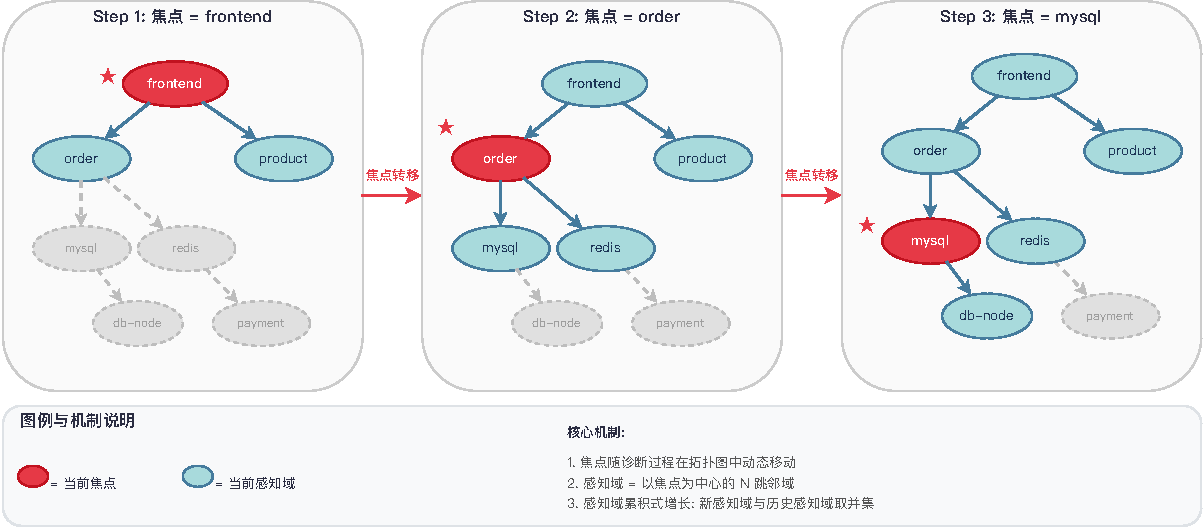
\includegraphics[width=\textwidth]{Figures-Src/Chap3-Methodology/focus-mechanism/chart.pdf}
    \bicaption{\enspace 焦点迁移与感知域变化示意}{\enspace Focus Shift and Perception Field Update}
    \label{fig:focus_mechanism}
\end{figure}

在上述机制下，观察智能体只能访问当前感知域内组件的指标、日志和链路数据，探索智能体也只能在当前感知域内切换分析对象，并可通过 \texttt{query\_status} 获取当前焦点与感知域状态。图\ref{fig:focus_mechanism}展示了焦点在系统拓扑中的迁移方式，以及感知域如何随着焦点变化而同步更新。例如，当当前焦点由支付服务切换为其数据库依赖链路上的某个组件时，系统会将该新焦点 $k$ 跳范围内相关的服务、容器和物理节点并入当前感知域；随后的观察与判断仍只在更新后的感知域内推进。通过这种方式，排查过程始终沿与当前路径直接相关的拓扑范围展开，从而兼顾在线执行效率与证据收集的有效性。

\subsection{SOP 驱动的多智能体在线诊断流程}

第3.4.2节从探索智能体与观察智能体的协同方式中抽象出了焦点与感知域这两个状态约束。进入在线阶段后，该约束由诊断智能体继承和执行。在完成故障指纹生成、SOP召回以及焦点与感知域初始化后，系统进入SOP驱动的在线诊断阶段。该阶段仍由诊断智能体与观察智能体协同完成，其运行方式在交互形式上与第3.3节中的离线探索过程相近：诊断智能体沿当前SOP节点逐步推进排查，观察智能体根据请求返回对应的指标、日志和链路证据，二者通过多轮交互不断缩小可疑范围。不同之处在于，第3.3节中的探索智能体服务于离线知识构建，其目标是在已知故障类型的前提下生成可用于构建SOP的执行轨迹；而本节中的诊断智能体服务于在线故障定位，其目标是利用召回的SOP，对当前故障逐步完成根因判断。

两类智能体虽然都与观察智能体配合完成任务，但它们分属不同阶段，面对的任务输入、输出结果以及对SOP的作用并不相同。表\ref{tab:exploration_vs_diagnosis}对这一差异作了简要对比。

\begin{table}[tbp]
    \centering
    \bicaption{\enspace 离线探索智能体与在线诊断智能体的角色差异}{\enspace Role Differences Between the Offline Exploration Agent and the Online Diagnosis Agent}
    \label{tab:exploration_vs_diagnosis}
    \renewcommand{\arraystretch}{1.2}
    \fontsize{10pt}{12pt}\selectfont
    \setlength{\tabcolsep}{4pt}
    \begin{tabular*}{\textwidth}{@{\extracolsep{\fill}}>{\centering\arraybackslash}p{2.0cm}>{\raggedright\arraybackslash}p{5.1cm}>{\raggedright\arraybackslash}p{5.1cm}@{}}
        \toprule
        \rowcolor{lightgray!30}
        \textbf{比较维度} & \textbf{探索智能体（离线）} & \textbf{诊断智能体（在线）} \\
        \midrule
        所属阶段 & 离线知识构建阶段 & 在线故障诊断阶段 \\
        \midrule
        任务前提 & 已知故障类型先验，不可见真实故障位置 & 仅有当前故障观测数据，由故障指纹召回初始 SOP \\
        \midrule
        核心职责 & 围绕可疑组件、传播路径与竞争候选展开探索，生成完整排查轨迹 & 围绕当前 SOP 节点收集证据、判断条件并逐步收敛根因 \\
        \midrule
        与 SOP 的关系 & 在当前 SOP 上导航或逃逸扩展，为 SOP 构建与修订提供依据 & 以召回 SOP 为执行约束，必要时触发逃逸机制扩展诊断路径 \\
        \midrule
        输出结果 & 带标签的 SOP执行轨迹 & 根因诊断结论及其证据链 \\
        \midrule
        对知识库的作用 & 直接作为决策单元提取与 RuleAgent 更新的输入 & 经人工审核后补全为新故障实例，触发故障指纹与 SOP 增量更新 \\
        \bottomrule
    \end{tabular*}
    \setlength{\tabcolsep}{6pt}
\end{table}

与离线探索不同，在线诊断开始时，系统输入只有当前故障的指标、日志和调用链路数据。故障指纹召回返回的是一个可作为起点的 SOP，而不是最终答案。诊断智能体仍需结合观察智能体返回的证据，持续判断当前节点对应的诊断假设是否得到支持、是否需要沿现有分支继续排查、是否应切换到其他节点，或者是否需要在当前 SOP 无法解释现象时触发逃逸机制。在线阶段的重点在于利用已有 SOP 尽快使诊断过程收敛到可信的诊断结论。

具体而言，在线诊断过程同时受到当前 SOP 节点、当前焦点和已收集证据三项信息的共同约束。当前 SOP 节点给出此时应执行的检查任务，当前焦点限定此时优先排查的组件实例，观察智能体返回的证据则用于判断当前节点对应的验证条件是否满足，以及后续应继续沿现有 SOP 推进、在 SOP 内切换分支，还是触发逃逸机制扩展新的排查路径。为便于说明，本文将 SOP 驱动的在线诊断过程概括为以下四类关键操作：

\begin{enumerate}[label=（\arabic*）]
    \item \textbf{证据收集与更新。}
    当诊断智能体到达某一 SOP 节点后，首先根据该节点对应的诊断意图、当前焦点以及已有证据，确定本轮需要观察的组件对象与证据类型，并向观察智能体发出诊断请求。观察智能体随后在当前感知域内收集相应的指标、日志和调用链路数据，并将其整理为可供后续判断的结构化证据。随着新证据不断加入，系统对当前故障状态的刻画也随之更新，为后续路径判断提供依据。

    \item \textbf{SOP 内分支导航。}
    若新收集到的证据尚不足以支持沿当前节点的主分支继续推进，但已能够表明当前检查方向不成立，且现有 SOP 中仍存在其他可供验证的分支，则诊断智能体不会立即脱离当前 SOP，而是在当前 SOP 内转向其他候选检查路径。此时，系统仍保持当前感知域约束，仅在已有 SOP 覆盖的范围内调整排查方向，从而优先利用已沉淀的诊断知识完成进一步定位。

    \item \textbf{条件满足后的节点转移。}
    若当前证据能够支持某一分支条件成立，则诊断智能体沿满足条件的边转移到下一节点，并据此更新当前检查任务与焦点位置。节点转移意味着诊断过程在现有 SOP 上取得了进一步收敛：系统不再停留于当前局部判断，而是将排查推进到下一步更具体的验证环节。随着节点不断转移，诊断过程逐步缩小可疑范围，并向最终根因结论逼近。

    \item \textbf{逃逸机制触发。}
    若当前 SOP 中不存在与现有证据相匹配的后续分支，或者在当前局部范围内持续收集证据后仍无法形成有效判断，则说明现有 SOP 尚不足以覆盖当前故障场景。此时，系统触发逃逸机制，在当前路径基础上扩展新的排查方向，并围绕新的候选对象继续收集证据与推进判断。逃逸并不意味着放弃 SOP，而是在既有知识无法解释当前现象时，对未被覆盖的诊断路径进行补充性探索，以避免诊断过程停滞在现有结构边界处。
\end{enumerate}

在上述四类操作的交替推进下，诊断智能体与观察智能体通过多轮协同不断缩小可疑范围，并最终形成针对当前故障的诊断结果。在线诊断结束后，诊断智能体提交候选故障位置、候选故障类型及其对应的关键证据链，作为后续人工审核与知识库增量更新的输入。

\subsection{在线诊断结果审核与知识库增量更新}

在线诊断阶段的直接输出，是由诊断智能体在完成排查后提交的诊断结果，其中包含候选故障位置、候选故障类型以及支撑这些判断的证据链。该结果不宜在未经审核的情况下直接纳入知识库，因为线上故障的故障位置和故障类型需要在排查过程中逐步判断，仍可能存在误判。例如，系统诊断智能体可能将故障诊断为“数据库连接池耗尽”，但实际处置后发现根因是“慢查询导致连接堆积”。如果不经过人工审核就直接更新知识库，就会将错误案例引入历史故障数据，进而影响后续故障指纹召回与 SOP执行效果。

因此，诊断结果仍需由人工结合实际处置过程、业务恢复情况、组件修复记录以及必要的事后分析进行审核。只有当人工审核确认该结果与实际处置情况一致后，它才会被确认为新的在线故障实例。经确认后的在线故障实例会重新进入前两节给出的知识沉淀过程：一方面，系统按照第3.2节的方法为该实例生成故障指纹，并判断其应归入现有故障簇还是形成新的故障簇，从而更新故障指纹库及其聚类结果；另一方面，系统按照第3.3节的方法围绕该实例补充 SOP执行轨迹，提取新的决策单元并计算权重，再基于规则对现有 SOP 进行增量修订。这样可以避免把单次在线结论中的偶然现象或临时处置动作直接固化为通用流程。


%---------------------------------------------------------------------------%
%->> 3.5 本章小结
%---------------------------------------------------------------------------%
%---------------------------------------------------------------------------%
%->> Section 3.5: 本章小结
%---------------------------------------------------------------------------%

\section{本章小结}

本章说明了诊断经验如何转化为可执行的知识。第3.2节将指标、日志和调用链路统一编码为故障指纹，用于相似故障检索。第3.3节通过带故障类型先验的离线探索生成 SOP执行轨迹，再从轨迹中提取带权决策单元，并在当前版本 SOP 上完成增量修订。第3.4节给出了在线阶段的执行方式：系统先通过故障指纹召回相应 SOP，再在焦点与感知域约束下推进排查；若现有 SOP 无法覆盖当前场景，则通过逃逸机制进行路径探索，并将人工复核确认的新故障实例回流离线流程。下一章将在此基础上介绍平台的设计与实现。

